\documentclass[12pt,a4paper]{report}
\usepackage[utf8]{inputenc}
\usepackage[T1]{fontenc}
\usepackage{microtype}
\usepackage{graphicx}

\usepackage{cite}
\usepackage{upgreek}
\usepackage{amsfonts}
\usepackage{amsmath}


%SPACING
\linespread{1.2}


%%% STYLE OF PAGES NUMBERING
\pagestyle{plain}


\begin{document}

\pagestyle{empty}
\begin{center}
{\Large \textbf{Webs on trees}\\}
{\large \textbf{Understanding ecological network motifs through phylogenetics trees and backward\\}}
\vspace{1cm}
{\large 
Giulio Valentino Dalla Riva\\
\vspace{0.5cm}
Supervisors: \\
Prof. Mike Steel (Mathematics and Statistics)\\
Prof. Daniel Stouffer (Biology)}\\
\end{center}

\begin{figure}[h]
	\centering
		
\includegraphics[width=0.5\textwidth]{images/UClogo}
\end{figure}

\vspace{1cm}
\begin{center}
{\large  
Research Proposal for the Degree of Doctor of Philosophy\\
in the Department of Mathematics and Statistics\\
University of Canterbury\\
\vspace{0.3cm}
$\cdot$ 2013 $\cdot$}
\end{center}
\vspace{1cm}
\tableofcontents

%%%---%%%---%%%---%%%---%%%---%%%---%%%---%%%---%%%---%%%---%%%---%%%---%%%
%%%---%%%---%%%---%%%---%%%---%%%---%%%---%%%---%%%---%%%---%%%---%%%---%%%
\chapter{Introduction}

The anthropogenic pressure on the landscape and the living species communities is every day more evident. The biodiversity of the world is recognized as a precious, yet fragile, treasure and more and more efforts are done in order to preserve it, both in the local and in the global scale. A sensible conservation policy requires science to understand the current status of the ecological world and to develop tools with which to forecast its future status.

Biodiversity is, at the same time, the product of fast time processes, such as the one ruling the dynamics of the web of life, and long time processes, such as the ones involved in the growth of the tree of life.

Hence, it is of great importance to understand how this different time scale processes interact.

We approach the problem of studying the interplay between the building blocks of structures of the web and tree of life: motifs. In foodwebs, motifs are given by small subgraphs, which are seen to be over-abundant in the empirical observed webs. In phylogenies we can focus our attention on the mutual evolutionary distance between pair, triplets, quadruplets, ... of species.

In this scenario many elementary question, regarding trophic linking, speciation or extinction events, are yet to be answered.

We will explore the interplay between webs and trees following different approaches, including statistical description, model development and analytical investigation.



\chapter{State of the art}
Foodwebs are currently analysed in ever growing detail: a number of network characteristics are considered of particular ecological interest - e.g., connectivity, stability, keyroles, degree distribution, motifs distribution. Analogously, phylogenetic trees also topical and their reconstruction is becoming sounder and sounder thanks to the developing sequencing techniques. The relationship between trophic networks and phylogenies is studied within different approaches including statistical descriptions, modelling efforts and analytical studies.

The evolutionary history of a species ensemble has non trivial influence on the species' role in the food webs, as shown by Stouffer et al. \cite{stouffer_evolutionary_2012}, Naisbit et al. \cite{naisbit_phylogeny_2012}. Moreover, Ekl\"{o}f et al. \cite{eklof_relevance_2012} showed that the taxonomy of a species community is a valid predictor of its trophic interactions: the authors find, indeed, a phylogenetic signal in the formation of food webs; similar results are found in Krasnov et al. \cite{krasnov_phylogenetic_2012}, Ives et al. \cite{ives_phylogenetic_2006}, Bersier et al. \cite{bersier_signature_2008}.

Interpretations of motifs in terms of ecological properties has been reviewed by Bascompte and Stouffer \cite{bascompte_assembly_2009}, while various field investigations have been and are being attempted (see for example Rip et al. \cite{rip_experimental_2010}). It has been argued that Phylogenetic Diversity arising from the evolutionary history of a species community may be a predictor of ecosystems functions: see  Srivastava et al. \cite{srivastava_phylogenetic_2012}, Gravel et al. \cite{gravel2010experimental}, Mouquet et al. \cite{mouquet2012ecophylogenetics}.

\paragraph{Modelling}
A survey of classical models, up to the models developed in 2002, can be found in Drossel and McKane \cite{drossel_modelling_2002}. The author focused on stability issues, covering both static and dynamical models. More recently, a number of models can be found in Pascual and Dunne \cite{pascual_ecological_2005}.

Drossel and McKane proposed a model taking into account predator-prey dynamics (see \cite{drossel_influence_2000, mckane_models_2005} and references within) implementing Arditi-Ginzburg Predator-Prey ratio-dependent efforts \cite{arditi_coupling_1989} and traits evolution (the proportion of a prey $p$ in a predator $P$'s is given as the score of a traits matching matrix). In \cite{quince_topological_2005} they implemented other predator-prey dynamics, e.g., Lotka-Volterra, and observed that the model food web outcome didn't fit the empirical observed data. The model has been developed in order to study immigration-speciation processes \cite{powell_comparison_2009}, and complexity-stability relation \cite{plitzko_complexitystability_2012}.

Caldarelli and Garlaschelli proposed a general framework for the ecological network evolution, the Webworld model \cite{caldarelli_modelling_1998}. Cannon et al. introduced a Lotka-Volterra niche model starting from a void universe with a single steady source of biomass \cite{cannon_diversification_2010} and gave an interpretation of two peculiar motifs in terms of network expansion within total biomass constraint. A food web model implementing niche model and the hypothesis that speciation and extinction rates decrease with increasing body mass was proposed in 2005 by Rossberg et al. \cite{rossberg_explanatory_2005} and then further developed \cite{rossberg_food_2006} implementing the signal of an evolutionary history where new species avoid to compete with their ancestors.

It would be useful to reconstruct foodwebs structure along their historical evolution. Although detailed direct observations are yet to come, some attempts have been done, see Roopnarine et al. on paleocommunities \cite{roopnarine_networks_2010, roopnarine_red_2012} or Dunne et al. for the Cambrian period \cite{dunne_compilation_2008}. Another possibility has been introduced by Doi et al. \cite{doi_shorter_2012}: the author examined lakes spanning six order of magnitude different ages, and hence showing the result of shorter or longer evolution times.

\paragraph{Extinction events, hybrids and Phylogenetic Diversity}
Extinction events prune the trees of life. This results in a loss of phylogenetic diversity, which depends clearly on which species goes extinct and which are retained.

A basic model which is widely used to predict on the future biodiversity of a species community under extinction threat is the Field of Bullets model, introduced by Raup in 1984 \cite{raup1984evolutionary}. Since its introduction the model has been variously generalised and applied with good results.

An immediately related problem asks, under limited resources, to find a conservation policy maximizing the expected biodiversity. A first answer comes from just considering the number of saved species. Prioritizing the length of the saved branches means taking into account Phylogenetic Diversity (Faith \cite{faith1992conservation}): this approach was introduced by Witting and Loeschcke \cite{witting1995optimization}.

Weitzmann \cite{weitzman1998noah} considered probabilities of survival and budget limitation and introduced the so-called "Noah's Ark Problem". Hartmann and Steel \cite{hartmann2006maximizing} showed that, under certain limitation, we can optimally solve the problem through a greedy algorithm.

Bordewich and Semple \cite{bordewich2008nature} considered an important generalization of the Noah's Ark Problem where conservational policy can be applied to groups of species, or nature reserves, hence introducing relationship between the survival probability of different species.

Recently, Billionnet \cite{Billionnet01012013} showed that fast mixed-integer linear programming techniques can give a near-optimal solution to both the original Noah's Ark Problem and its nature reserves generalization. This techniques also yield an upper bound to the optimal solution.

With a different approach, a relationship between the survival probability of species taking into account their phylogenetic diversity (in terms of shared common evolutionary history) was introduced as a trait-based extinction model, introduced by Steel and Faller \cite{steel2009markovian, faller2012trait}: the model allowed trait evolution along the tree branches following a markov chain model.

An explicit introduction of ecological constraints into a field of bullets extinction model has been proposed by Moulton et al. \cite{moulton2007optimizing}, where the authors used the concept of "viability", that is taking into account that every predator species has to predate at least on a species to survive. The model complexity has been studied by Faller et al. \cite{faller2011optimizing}.

\paragraph{Species stability}
Foodwebs have been described in terms of ecosystem stability under a perturbation regime ( which means, altering the population dynamic parameters, see for example Sol\'{e} and Bascompte \cite{sole2006self} for a recent overview). An usual approach is to consider linear or approximately linear population dynamics -- i.e., systems were the applied perturbation can be considered to produce a linear effect on the stable solution. As summarized by Sol\'{e} and Bascompte, ``Stability seems to be associated with diversity, but the exact nature of such association has been a matter of debates for decades'' and so it is currently, we can argue.

Working on protein transcription networks and neuron networks, Prill et al. \cite{prill2005dynamic} gave a numerical characterization of 3-motifs and 4-motifs in terms of stability through a Structural Stability Score, defined as the probability that the dynamical system corresponding to a given motif relaxes monotonically to the stable equilibrium after a small linear perturbation. Significantly the authors found a positive correlation between the SSS score of a motif and its over or under representation in an empirical network.

\chapter{Research objectives and approach}

We aim to discover the relationship between phylogenetic evolution and foodweb evolution.

A main focus of the thesis trying to disentangle the correlation between basic trophic network structural elements, such as elementary predator-preys linking, foodweb motifs, node or edge roles (as depicted in figure~\ref{fig:motifs}), and phylogenetic tree properties, such as phylogenetic diversity, pairwise distance between leaves, clades and clans. In this scenario, some foundational question are yet to be answered.

\begin{figure}[h]
	\centering
		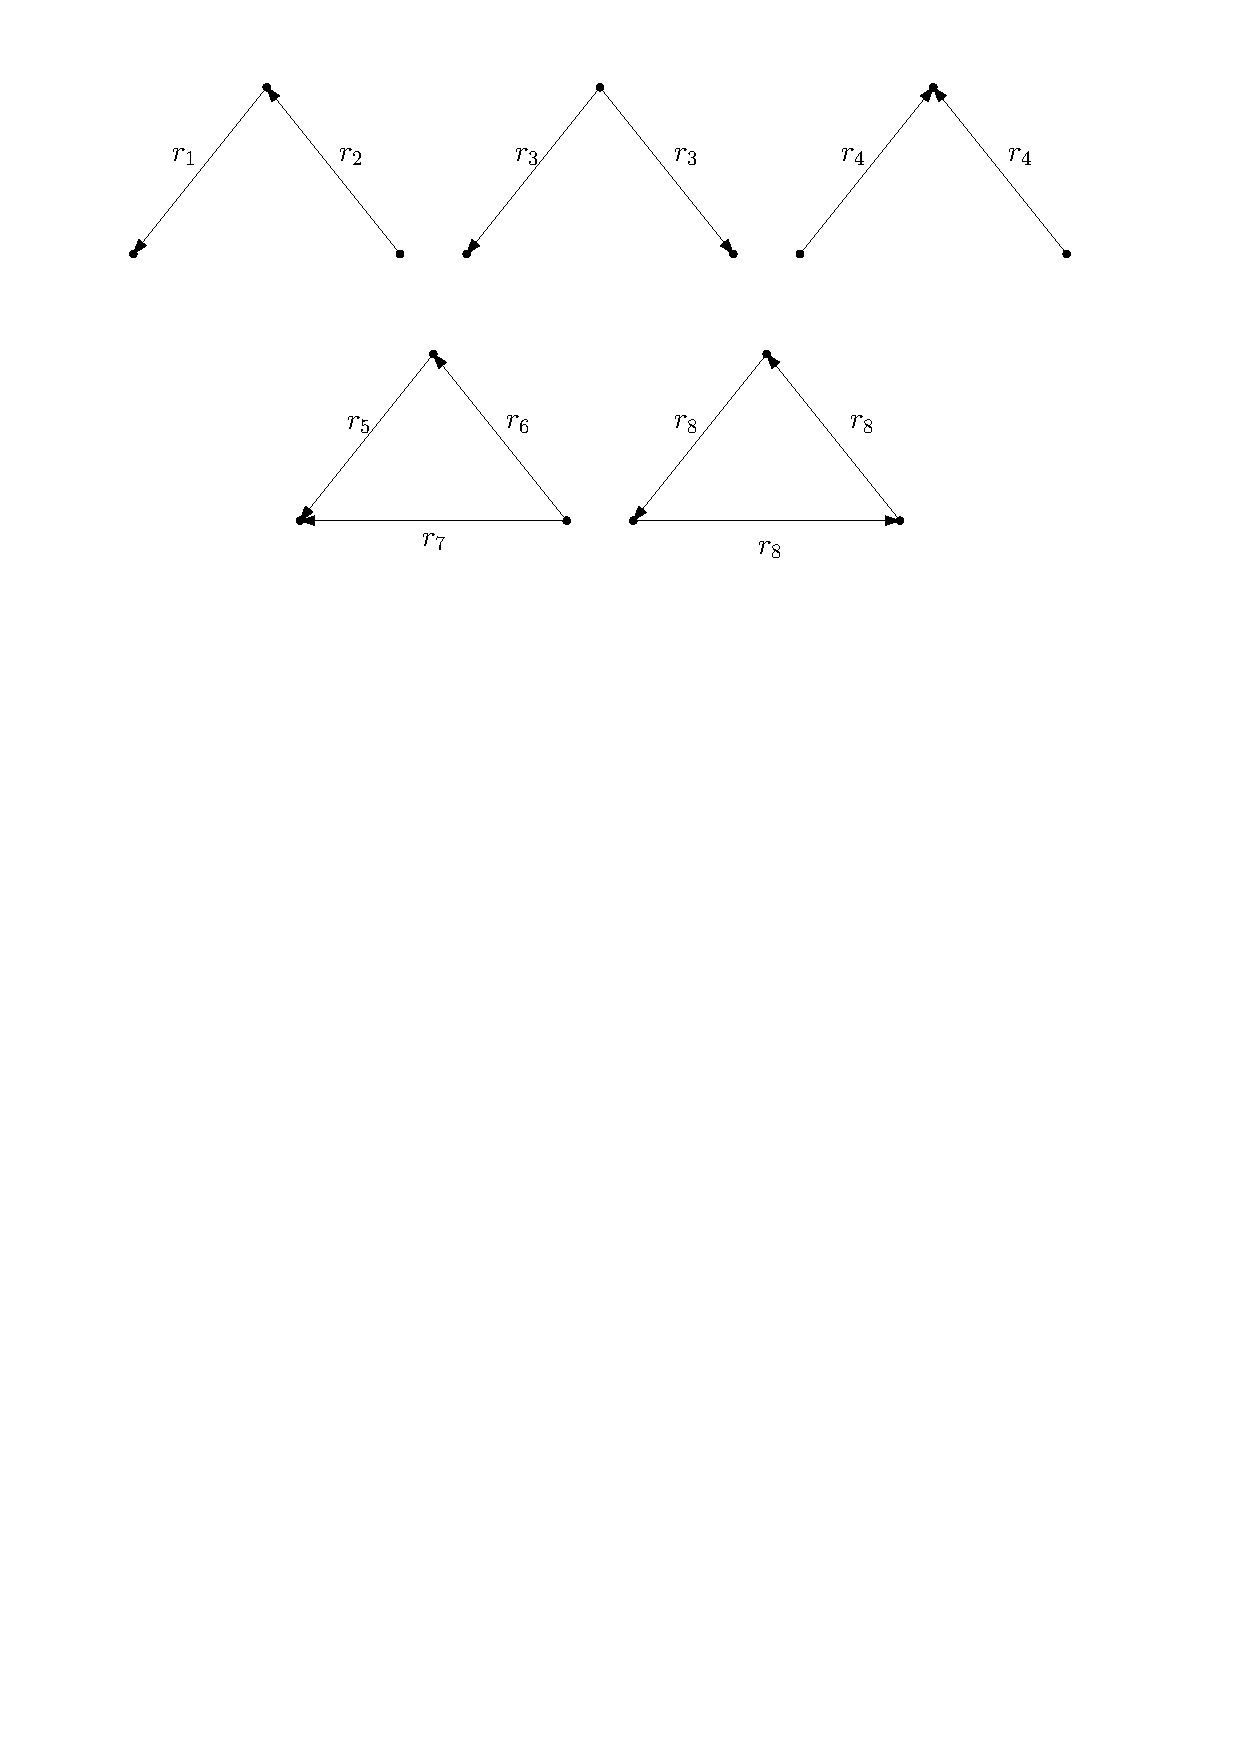
\includegraphics[width=0.6\textwidth]{images/motifs}
		\caption{The different edge roles in the five most common predation motifs.}
		\label{fig:motifs}
\end{figure}


One problem, that will need to be solved, arises from the merging of data coming from two different empirical sources: genetic sequencing studies and foodwebs observation. The usual empirical data are given in the form of an ecological community which phylogeny is reconstructed and the species are mapped in a foodweb. This gives a straightforward mapping of the phylogenetic tree leaves into the trophic relationship graph. The food can be variably detailed in terms of guilds census (how many extant species and trophic relationship are present in the given foodweb) and taxonomic resolution (how coarse is the identification of the guilds taxonomy). Analog uncertainty can be present in the phylogeny reconstruction, which may vary from a topological tree given by the taxonomic classification to a tree reconstructed from the actual genome sequencing of the observed species.


\section{Coupling ecological roles and phylogenetic structure}

\subsection{Foodweb and tree motifs}
Let $\uptau$ be the phylogenetic tree of the species in a certain ecological community and $\upomega$ its trophic relationship graph, the foodweb. Call $l_1, l_2, \dots , l_n$ the leaves of $\uptau$, we will use the same name to identify the species in the foodweb.\begin{figure}[h]
	\centering
		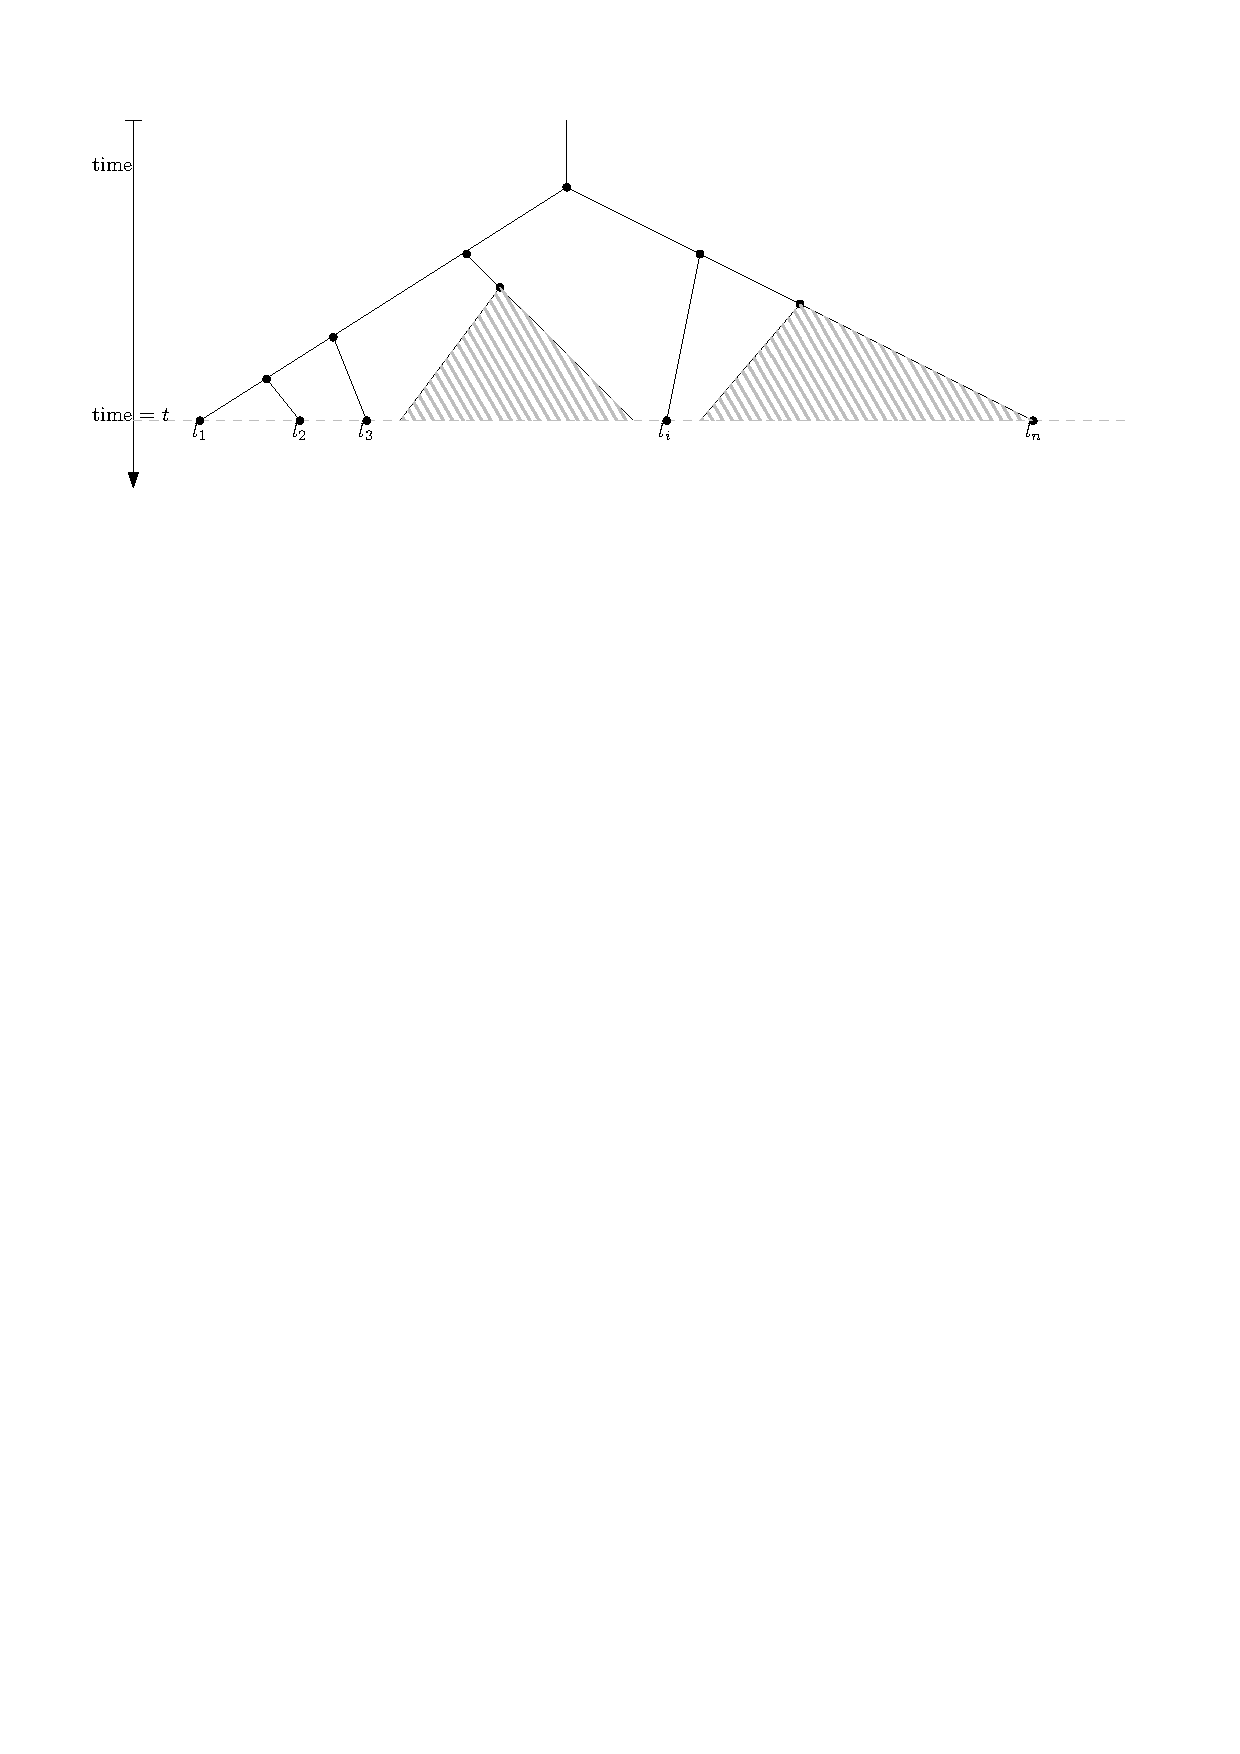
\includegraphics[width=0.8\textwidth]{images/phylogeny}
		\caption{A Phylogenetic Tree, the shadowed zones hides other branches and leaves.}
		\label{fig:phylogeny}
\end{figure}

We will express $\upomega$ in terms of its community adjacency matrix $M_{\omega}$ which elements $m_{\omega}^{ij}$ are equal to $1$ if and only if there's a link between node $i$ and $j$, and hence if and only if the species $l_i$ predates on the species $l_j$. Through the tree $\uptau$ we can define a phylogenetic distance matrix $M_{PD}$ which elements $m_{PD}^{ij}$ are given by the phylogenetic distance $Pd_{ij}$ between the species $l_i$ and $l_j$. As $Pd_{ij} = Pd_{ji}$, $M_{PD}$ is a symmetric matrix.
\begin{figure}[h]
	\centering
		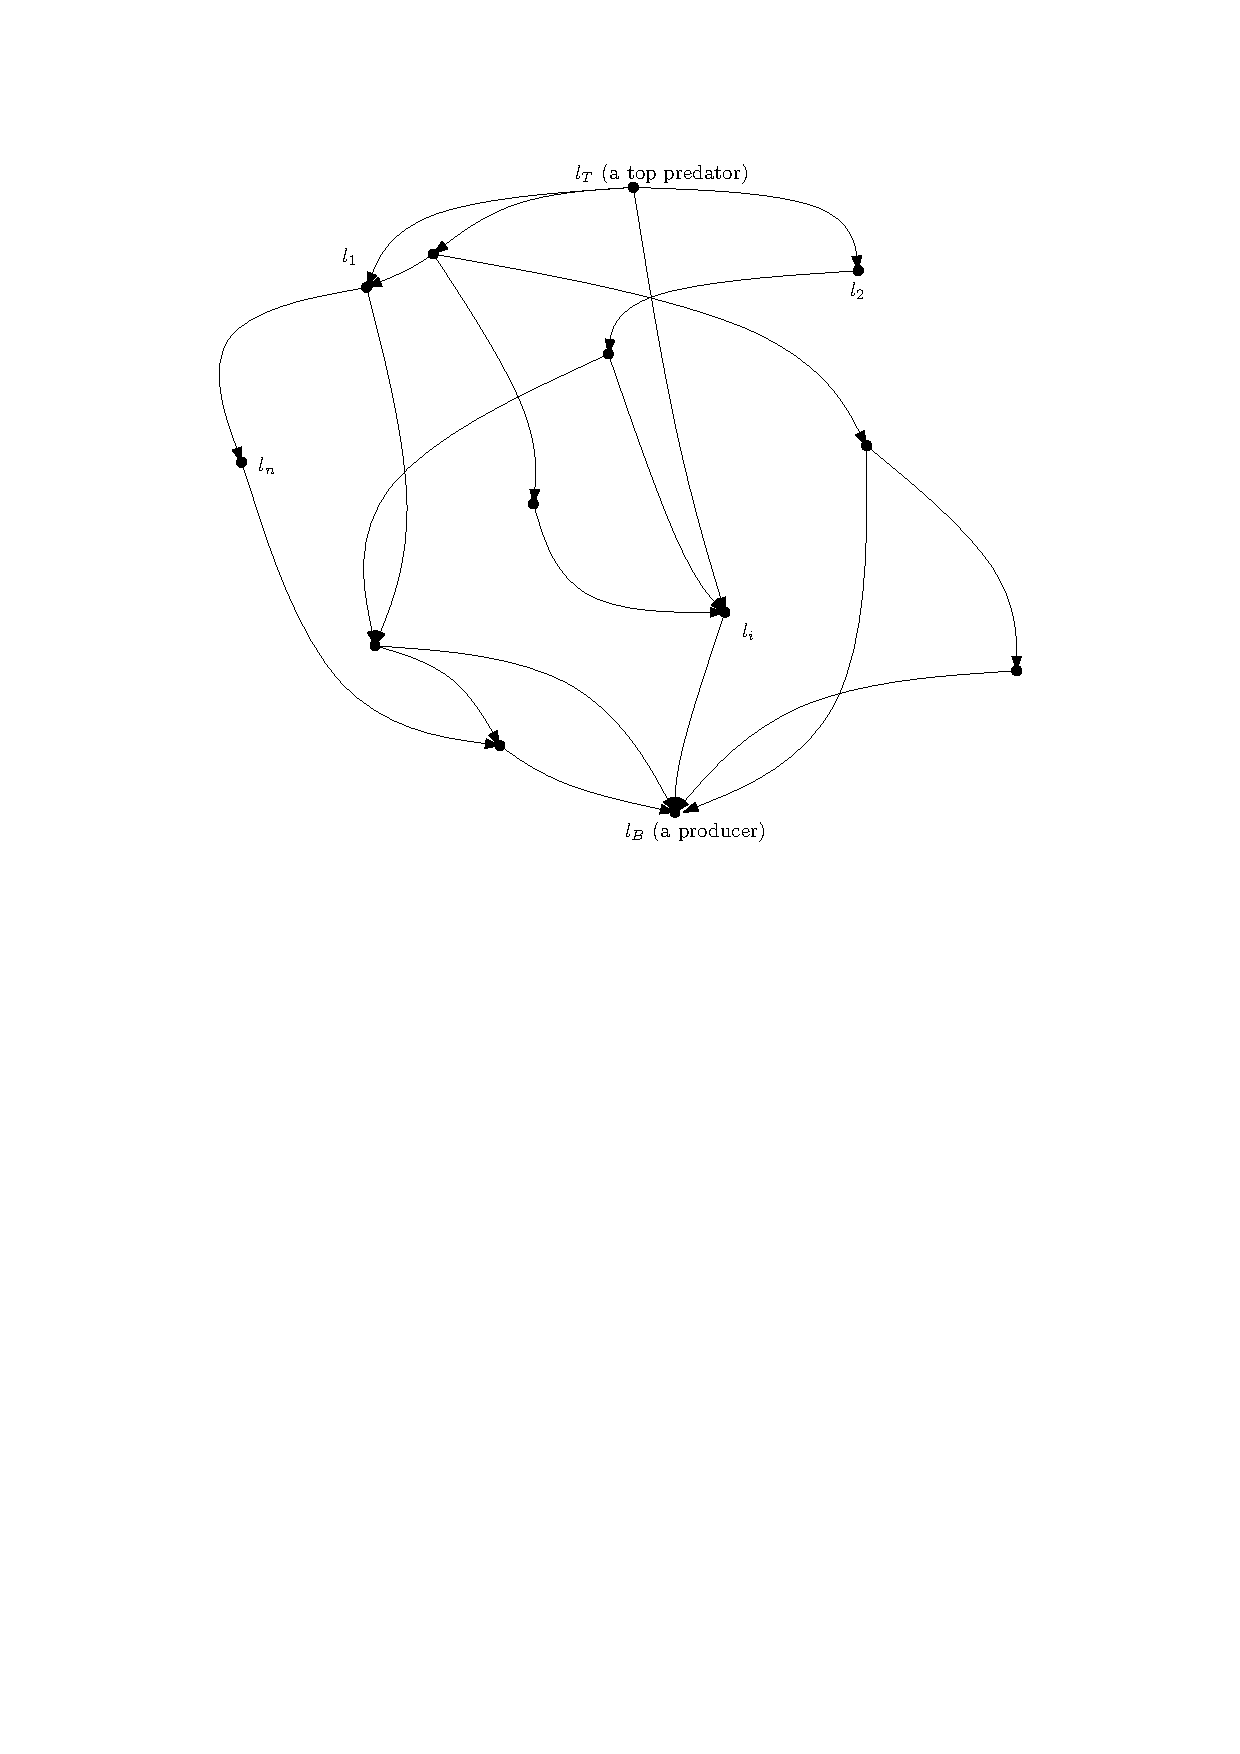
\includegraphics[width=0.5\textwidth]{images/foodweb}
		\caption{In this foodweb, and in all the proposal, we draw a link from a node $i$ to a node $j$ whenever species $i$ predates on$j$.}
		\label{fig:foodweb}
\end{figure}

The phenomenon we are looking at is apt to two complementary analysis approaches: 1) looking from the phylogeny to the foodweb structure, 2) looking from the foodweb structure to the phylogeny.

\paragraph{Couples}

We will consider basic components of both the predation network and the graph, starting with couples and adding one element at time.

\begin{enumerate}
\item What is the probability of $m_{omega}^{ij} = 1$ given that the species $l_i$ and $l_j$ have phylogenetic distance $Pd_{ij}=k$? Or, similarly, give a good approximating function \[f(k) \approx \mathbb{P}(m_{omega}^{ij} = 1 | Pd_{ij}=k ).\]
Notice that, in a model where evolution and predation are independent, we would have \[\mathbb{P}(m_{omega}^{ij} = 1 | Pd_{ij}=k ) = \mathbb{P}(m_{omega}^{ij} = 1) .\]

\item On the other hand, given $m_{omega}^{ij} = 1$, what is $\mathbb{E}\left[Pd_{ij}\right]$?
In a null model we have $\mathbb{E}\left[Pd_{ij} | m_{omega}^{ij} = 1 \right] = \mathbb{E}\left[Pd_{ij}\right]$.
\end{enumerate}

\paragraph{Triplets}
We will, then, study the identity mapping of foodweb elements triplets, called 3-motifs, into phylogenetic tree elements triplets, called triangles. We will call $\upomega(i,j,\dots)$ the subgraph induced by the node $i,j,\dots$.

We will call \emph{triangle of distances} a triplet $T_{ijk}=\{Pd_{ij},Pd_{jk},Pd_{ki}\}$ of mutual phylogenetic distances between three elements of the ecological community. Figure~\ref{fig:phylogenetictriplets} represents a triangle between the species $l_i, l_k, l_j$.

\begin{figure}[h]
	\centering
		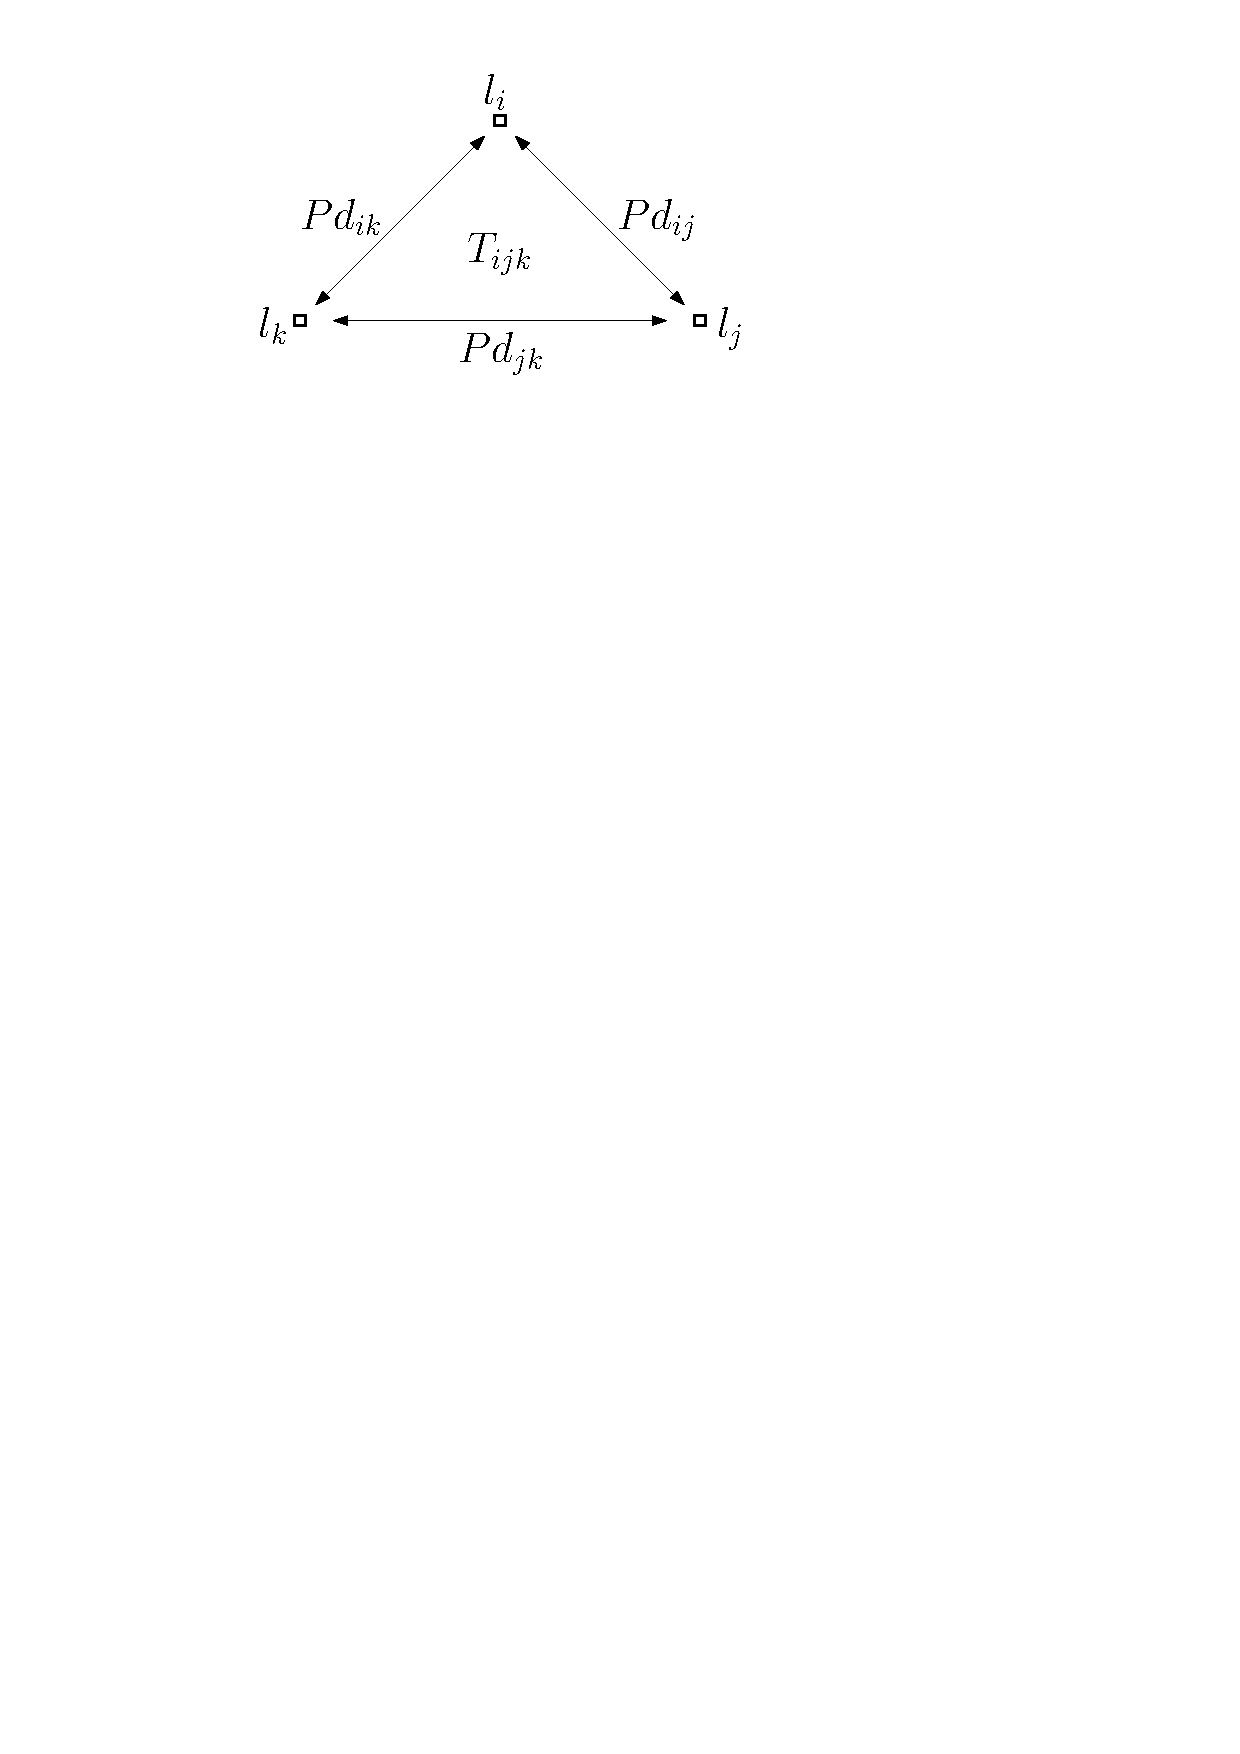
\includegraphics[width=0.3\textwidth]{images/phylogenetictriplets}
		\caption{A triangle of phylogenetic distances.}
		\label{fig:phylogenetictriplets}
\end{figure}

In the basic five 3-motifs, the ones without mutual predation relationship, we have 8 topologically different relationship $r_i$, as depicted in figure~\ref{fig:motifs}. If a connected subgraph $\upomega(i,j,k)$ is isomorphic to a certain motif with its edges in positions $r_z$, $r_{z'}$, $r_{z''}$ we will write \[\upomega(i,j,k) \to m(z,z',z'') \, .\]

The question 2) has now a straightforward extension: we want to give \[\mathbb{E}\left[T_{ijk}|\upomega(i,j,k) \to m(z,z',z'')\right].\]

The generalization of question 1) requires more attention.

We should notice that each predation relationship, the link $(i,j)$, can be part of various motifs including the species $l_i$, $l_j$ and a third species completing the motif, as shown in figure~\ref{fig:starij}.

\begin{figure}[h]
	\centering
		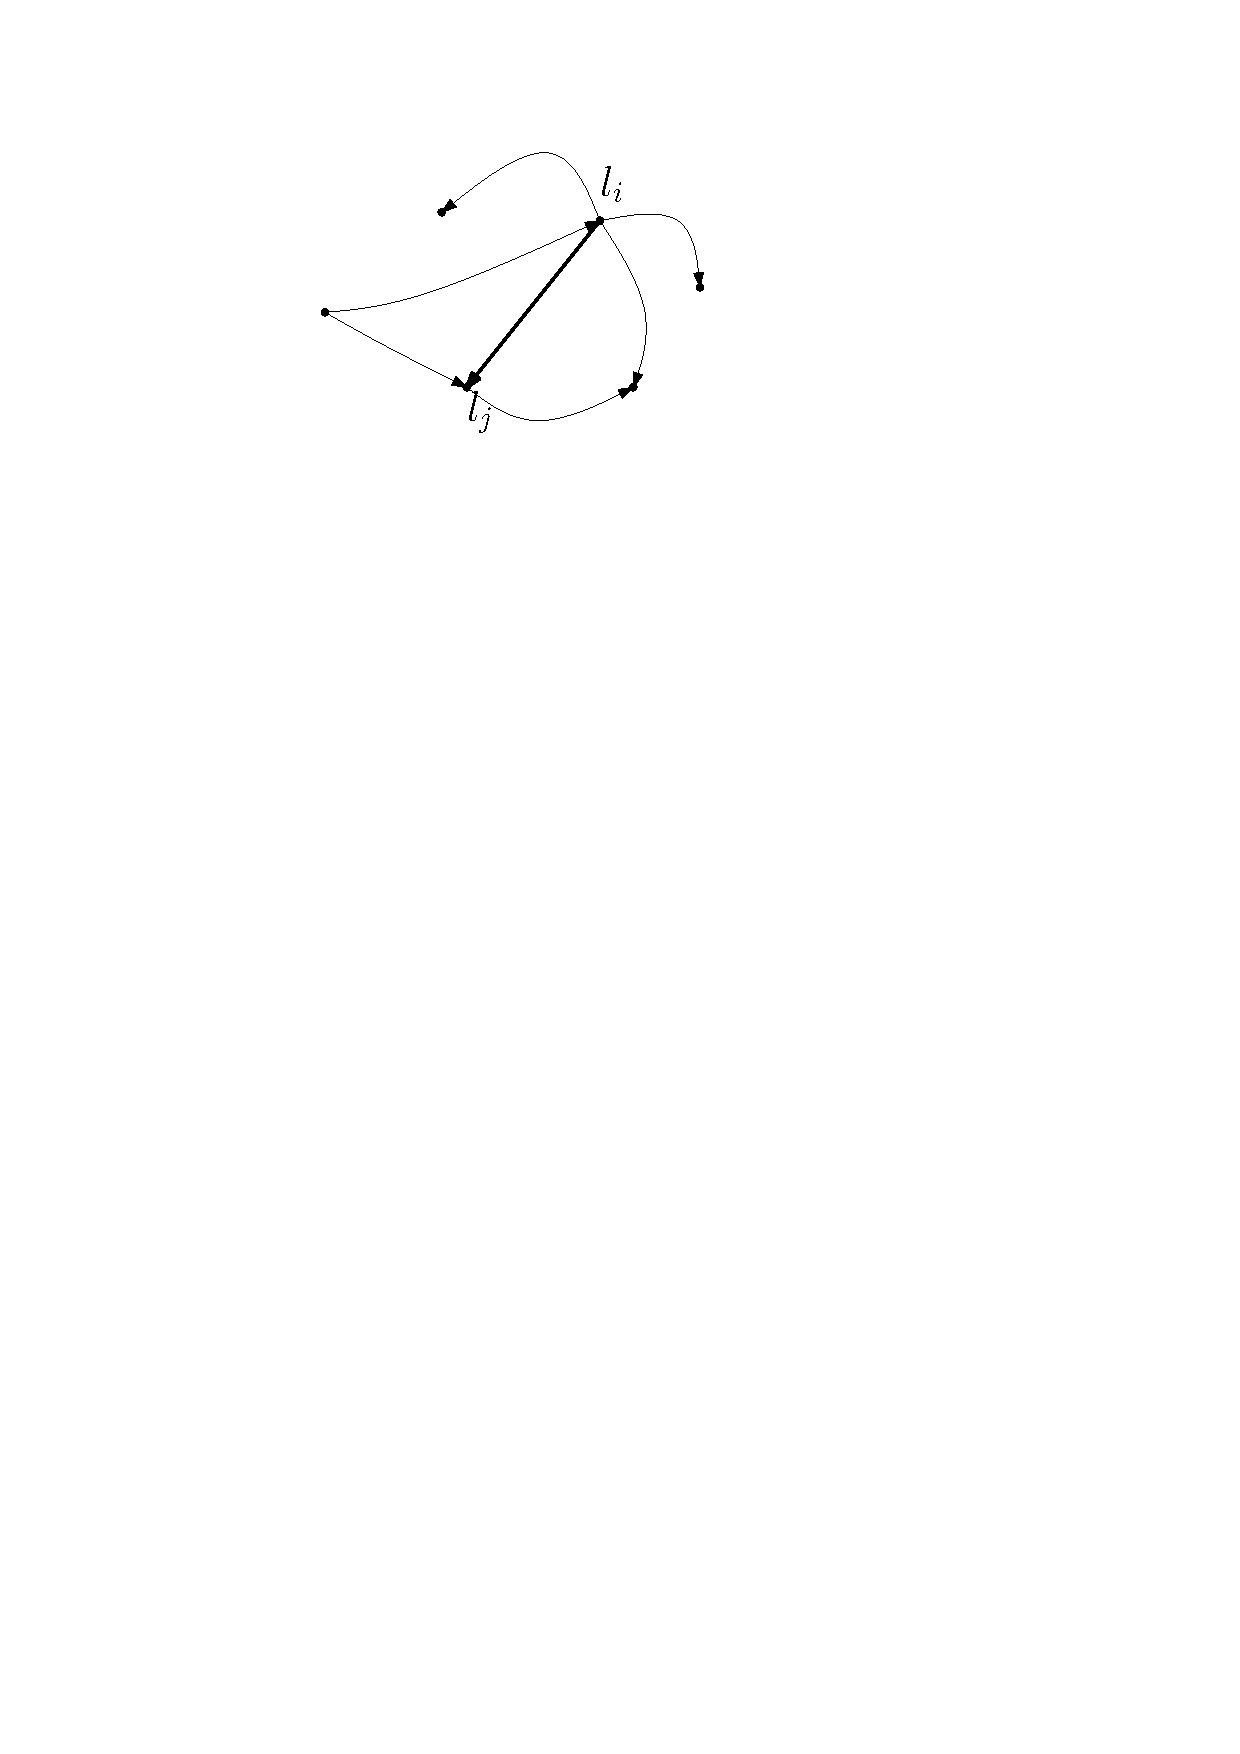
\includegraphics[width=0.3\textwidth]{images/starij}
		\caption{The neighborhood of the link $(i,j)$. In this example we will have $\underline{m}(i,j)=\{0,1,2,1,1,1,0,0\}$.}
		\label{fig:starij}
\end{figure}

We will call the \emph{motif distribution} of a link $(i,j)$ the vector $\underline{m}(i,j)=\{c_1,c_2,\dots,c_8\}$ where $c_i$ is given by the number of times the links $(i,j)$ occurs in position $r_i$. Each motif $\upomega(i,j,k)$ is associated to a triangle of distances $T_{ijk}$ and to each motif distribution $\underline{m}(i,j)$ is associated a vector of triangles $T_{\underline{m}(i,j)}$.

When considering the linking between two species in this scenario we should take into account also their 3-motifs neighborhood. Hence, the probability of having a predation relationship $(i,k)$ may be influenced by the phylogenetic distance between $l_i$ and $l_k$, the motif distribution such a relationship would have and all the triangles of distances induced by the motifs containing $l_i$ and $l_j$ if that relationship would exist.

Question 1) in this scenario asks: what's the probability of $m_{omega}^{ij} = 1$ given phylogenetic distance $Pd_{ij}=k$, motif distribution $\underline{m}(i,j)=\vec{v}$ and vector of triangles $T_{\underline{m}(i,j)}$. Or, similarly, give a good approximating function \[f(k,\vec{v},T_{\vec{v}}) \approx \mathbb{P}(m_{omega}^{ij} = 1 | Pd_{ij}=k, \underline{m}(i,j)=\vec{v}, T_{\underline{m}(i,j)}=T_{\vec{v}}).\]

Again, notice that, in a null model, the motif distribution should have no role.

\subsection{Does predation separate clans?}
Let's observe again a foodweb $\upomega$ and the phylogenetic tree $\uptau$ whose leaves set $L~=~\{l_1, l_2, \dots\}$ is a subset of the elements of $\upomega$. Explicitly denote the mapping of the leaves in $\upomega$ as $p(l_i)$. 

For each species $l_i$ we can define one couple of subsets in the foodweb and one couple in the phylogenetic tree. Indeed, we can split the neighbourhood of $p(l_i)$ in $\upomega$, which is denoted $\star(p(l_i))$, in the set of species predating $p(l_i)$, denoted $T(p(l_i))$, and the set of species $p(l_i)$ predates, $B(p(l_i))$. Hence $\star(p(l_i))= T(p(l_i)) \cup B(p(l_i))$. In a similar fashion, consider $l_i$ and the subset of $L$ given by the mapping of the species in $\star(p(l_i))$ into the phylogenetic tree, that is $p^{-1}(\star(p(l_i)))$, which we will denote as $\star(l_i)$. We define a rooted subtree by pruning all the species but the ones in $star(l_i)$ and placing the subtree root in $l_i$, which we denote  $\uptau_{|\star(l_i)}$. The subtree can be split in two principal clades, $C_r(l_i), C_l(l_i)$, such that $\uptau_{|\star(l_i)} = C_r(l_i) \cup l_i \cup C_l(l_i)$.

We can, at this point, ask what is the distribution of the predators and preys of $p(l_i)$ on the two clades $C_r(l_i), C_l(l_i)$.

As a working null hypothesis, let's assume the predation relationship is a random process independent from the evolutionary history. Consider a species $l_i$, in the foodweb $\upomega$. Suppose $l_i$ has in-degree $\delta^i(p(l_i))$ and out-degree $\delta^o(p(l_i))$. In- and out-degree of the species gives respectively the size of the $l_i$ predators set $T(p(l_i)$ and of the $l_i$ preys set $B(p(l_i)$. Predators and preys of $l_i$ are distributed uniformly at random on the leaves of $\uptau$. This means that, taking a leaf from $\uptau$, the probability of getting a $l_i$ predator, a $l_i$ prey or a species that as not direct trophic relationship with $l_i$ depends only the relative size of $L$, $B(p(l_i))$ and $T(p(l_i))$: drawing the lead uniformly at random or with a bias based on the tree structure doesn't change.

Calling $C_r(l_i)$ the larger of the two clans, the number of predators in it, which is the size of the set of leaves $C_r(l_i) \cap B(l_i)$,  will be distributed as a hypergeometric random variable. A similar reasoning can be proposed for the prey.

A more refined null model can be retrieved by considering the probabilistic niche model \cite{williams2010probabilistic} or the evolutionary niche model proposed by Ingram \cite{ingram2012should}: indeed, we can study the distribution of predators and preys on the two principle clades, assuming that, instead of being independent from the evolutionary history, the predation is shaped by a probabilistic niche model, where the niche position is a quantitative trait depending on the evolutionary history of the species.

Moreover, we can compare the model data with the data retrieved from the empirical observed network.


\section{Toward a simple speciation/predation model}

An insight into the mechanisms relating foodwebs evolution and speciation/extinction events can be acquired through the development of a suitable model which will be studied both from an analytical point of view and software  implemented.

Consider a certain ecological community given by a set of species $C_t$ at time $t$, let $\uptau_t$ be its phylogenetic tree at time $t$ and $\upomega_t$ its trophic relationship graph (the foodweb) at time $t$. Call $l_1, l_2, \dots , l_n$ the leaves of $\uptau_t$.

We will use the same naming also for the species in $\upomega_t$ without fear of confusion\footnote{In a more formal way we should introduce a bijective mapping $i$ of the leaves $l_i$ of $\uptau_t$ to the species $x_i$ in $\upomega_t$, so that $x_i=i(l_i)$.}.

\paragraph{Evolution event}

Each species $l_i$ can be chosen for a speciation event at the same rate $\sigma$. When the species $l_i$ is chosen at time $t$ for speciation it gives birth to two species $l_i'$ and $l_i''$, see fig.~\ref{fig:phylogenydeltat}. Hence, we will observe the building of a classical Yule random tree.

\begin{figure}[h]
	\centering
		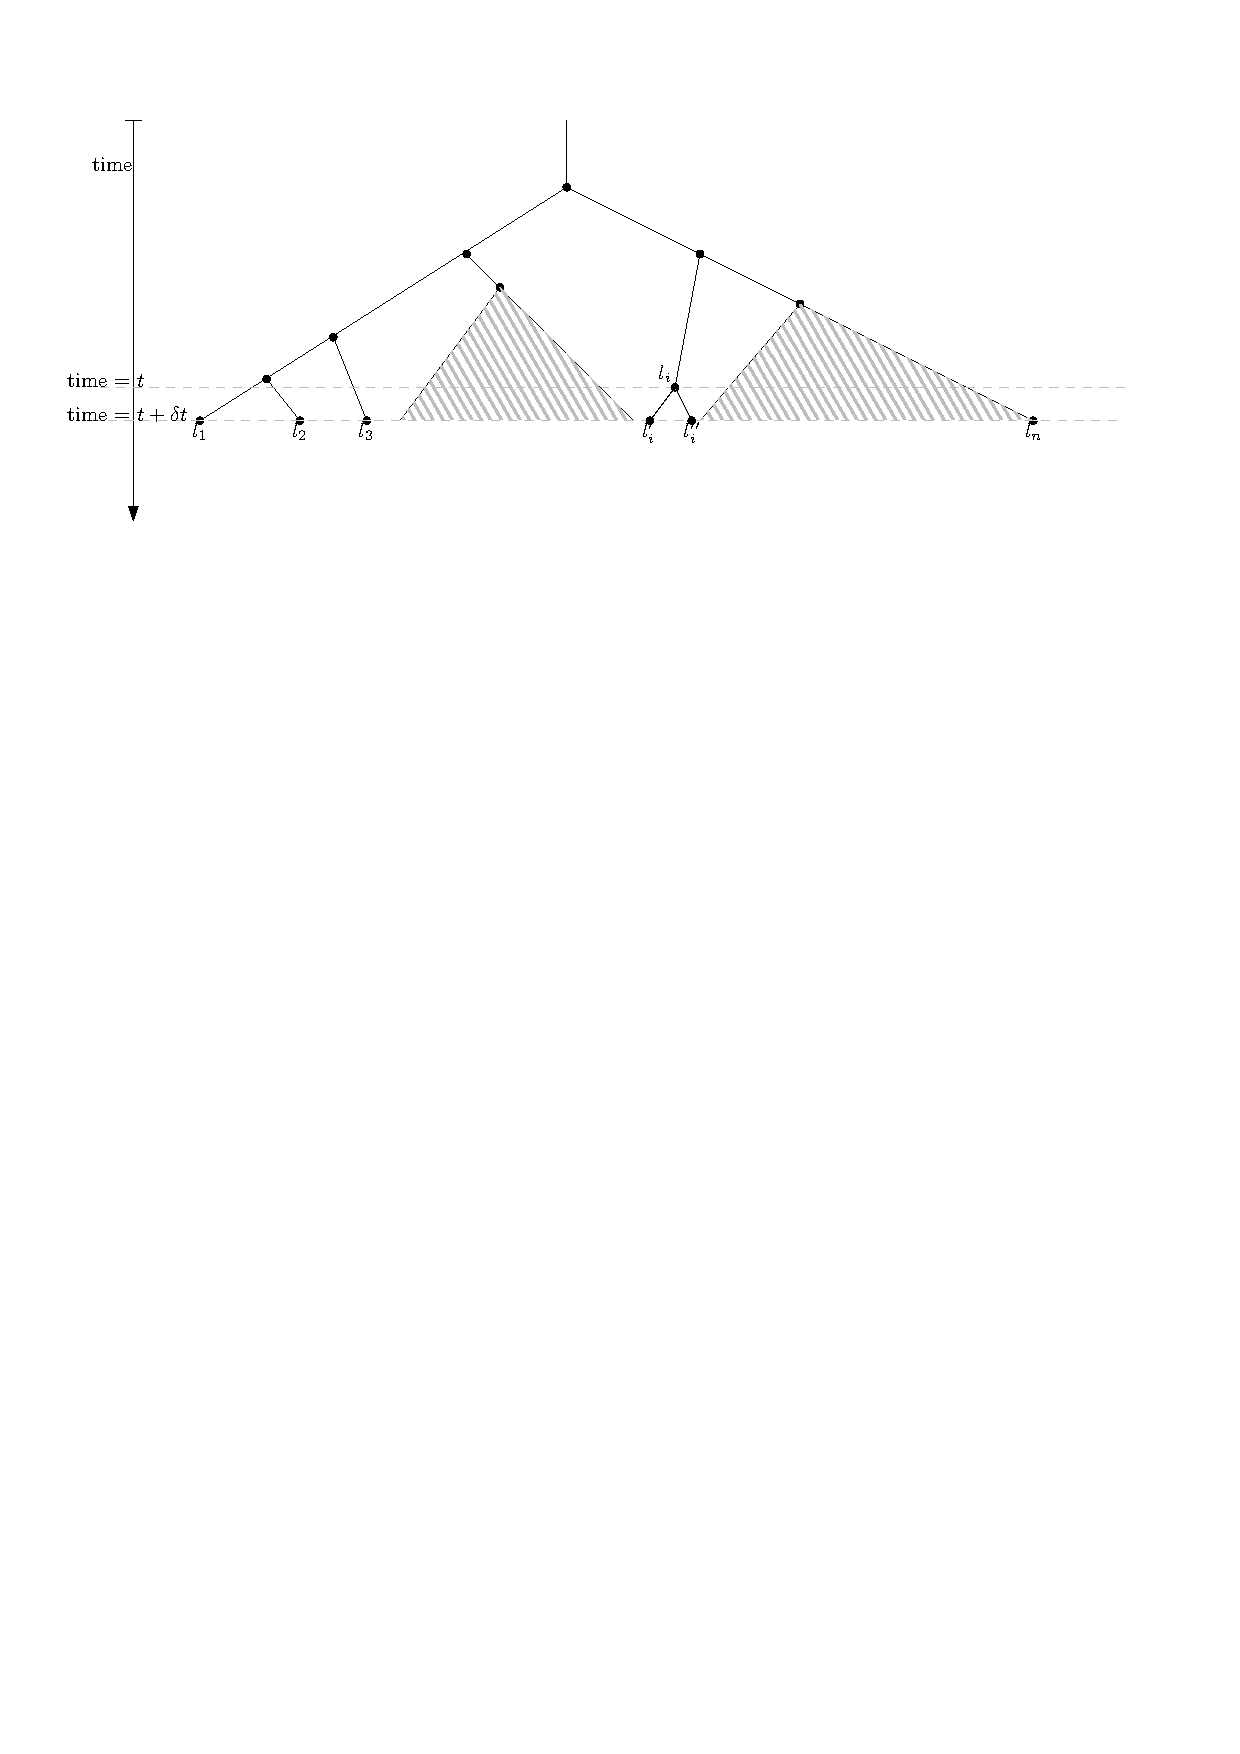
\includegraphics[width=0.8\textwidth]{images/phylogenydeltat}
		\caption{The phylogenetic tree $\uptau$ at time $t + \delta t$ has two new species, $l'_i$ and $l''_i$.}
		\label{fig:phylogenydeltat}
\end{figure}

\paragraph{Imperfect duplication}

To keep the model to the most simple case possible, we will assume that the place of one of the two siblings, $l_i''$, in $\upomega_{t + \delta t}$ will duplicate exactly the place of $l_i$ in $\upomega_t$. The other daughter will get rid of one of her ancestor predators with probability $p$ and, independently from this, will add one new prey to her diet with probability $q$.

In this model the predator will be drawn uniformly at random in the set $P(l_i)$ of the predators of $l_i$ and the prey will be chosen uniformly at random from $pp_{t}(l_i)$, which is the set of species $l_p$ in $C_t$ such that were no path from $l_p$ to $l_i$. Hence, we do not allow for the formation of predation chain relationship. The mechanism is depicted in figure~\ref{fig:fwspec1p}

\begin{figure}[h]
	\centering
		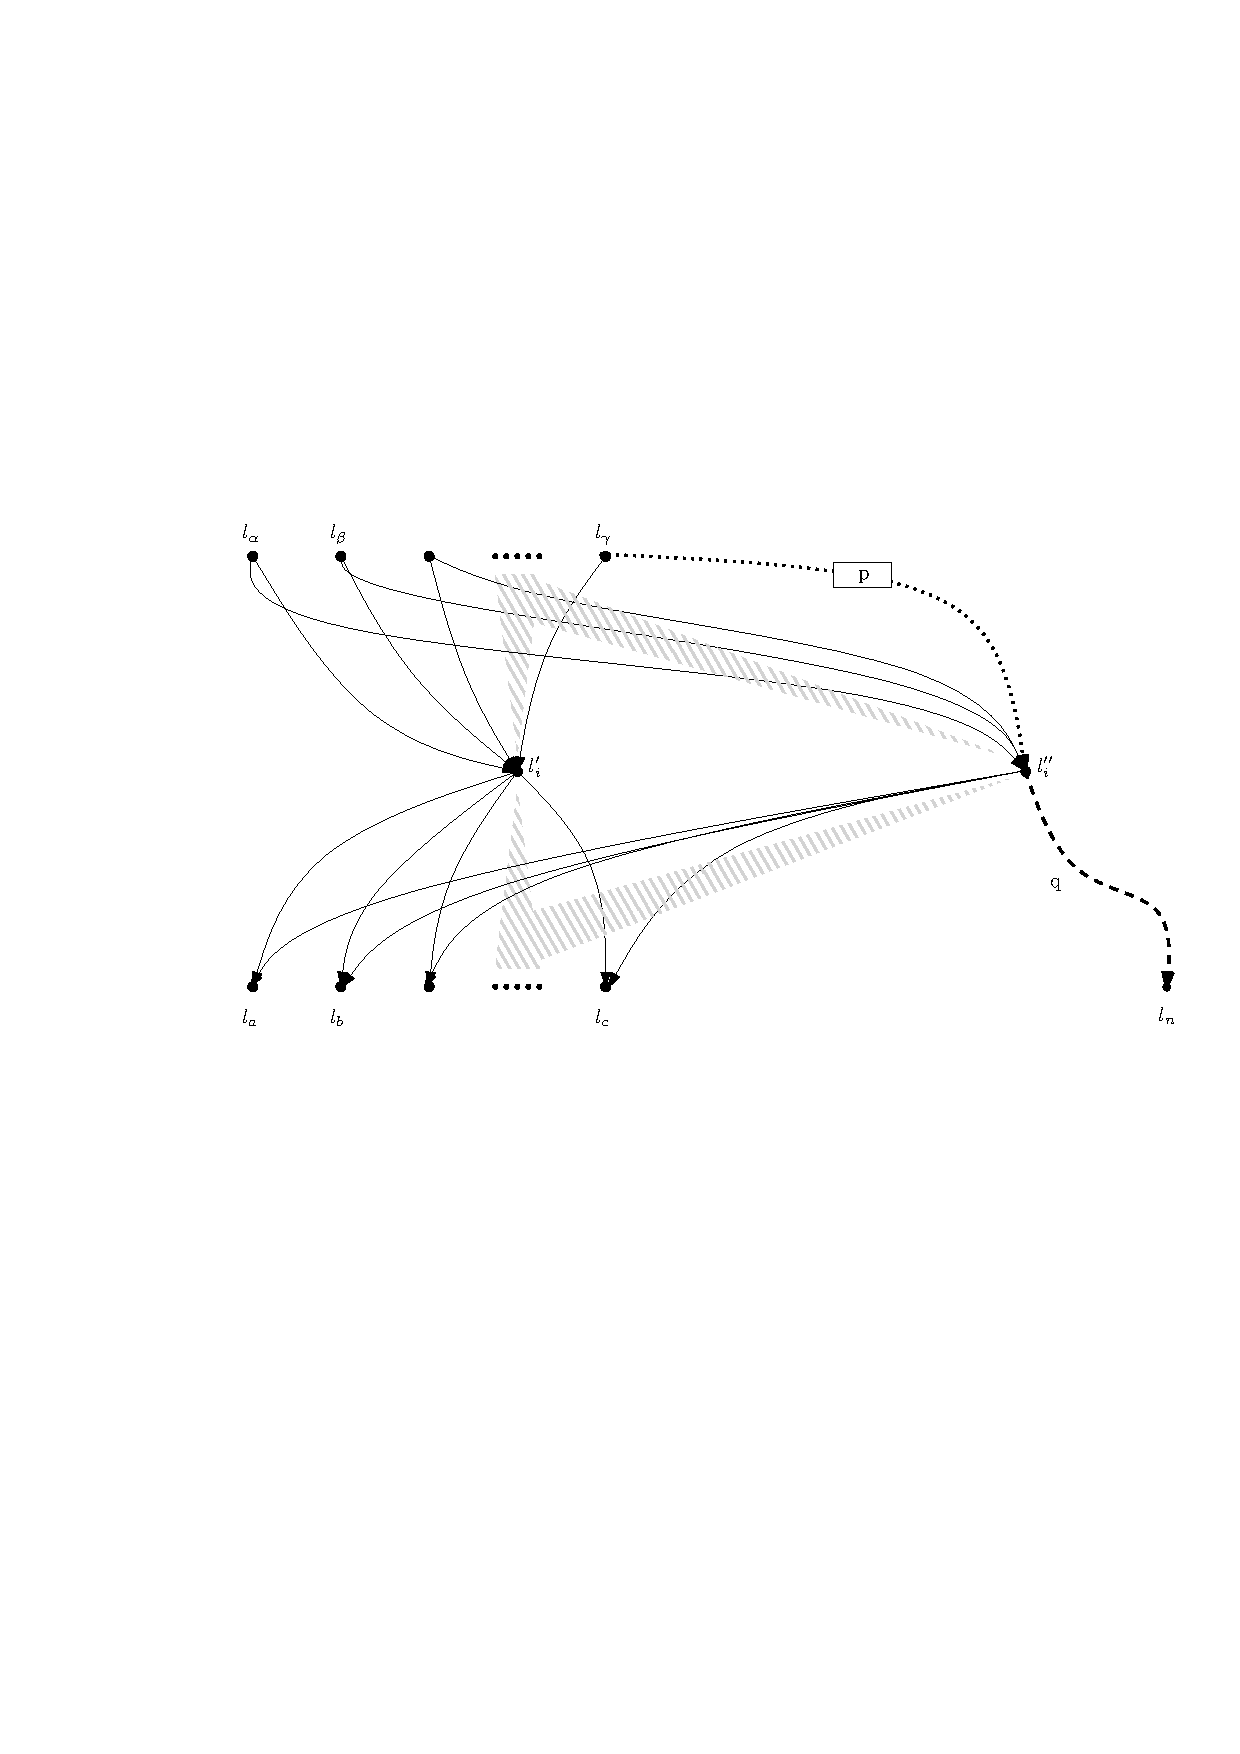
\includegraphics[width=0.8\textwidth]{images/fwspec1p}
		\caption{The rewiring of a species' foodweb neighbourhood during a speciation event in the imperfect duplication model.}
		\label{fig:fwspec1p}
\end{figure}

What happens to the in- (and out-) degree of the graph during a speciation event?

If both siblings just duplicated their mother, $$\delta^{in}_{l_i'}(t+\delta t)=\delta^{in}_{l''_i}(t+\delta t)=\delta^{in}_{l_i}(t) \, \, .$$ At the same time all predators of $l_i$ will acquire one more prey and all prey of $l_i$ will have one more predator.
Hence $$\delta^{in}_{tot}(t + \delta t) = \delta^{in}_{tot}(t) + \delta_{l_i}(t).$$

If $l_i'$ get rid of a predator, $l_i'$ in-degree decreases by one and the out-degree of the lost predator decreases by one. On the other hand, if $l_i'$ acquire a new prey, $l_i'$ out-degree increases by one and the in-degree of the new prey increases by one. Hence, if $l_i$ speciates at time $t$ and we don't have other speciation before $t + \delta t$, we have that

\begin{equation}
\mathbb{E}\left[\delta^{in}_{tot}(t + \delta t)\right] = \delta^{in}_{tot}(t) + \delta_{l_i}(t) + q - p
\end{equation}

which reduces, if $p = q$, to

\begin{equation}
\mathbb{E}\left[\delta^{in}_{tot}(t + \delta t)\right] = \delta^{in}_{tot}(t) + \delta_{l_i}(t) \, \, .
\end{equation}

Moreover, naming $\widehat{\delta^{in}}(t)$ the mean degree at time $t$, during one speciation event occurring in the interval $\left[t,t + \delta t \right]$, assuming no other speciation event happen in that time, and remembering that $\hat{\delta}(t)=2\widehat{\delta^{in}}(t)$ for each time $t$, we'll have that

\begin{equation}
\mathbb{E}\left[\widehat{\delta^{in}}(t + \delta t)\right] = \frac{(|C_t|+2)\widehat{\delta^{in}}(t)}{|C_t|+1} + \frac{q - p}{|C_t|+1}
\end{equation}

which reduces, for $p = q$, to

\begin{equation}
\mathbb{E}\left[\widehat{\delta^{in}}(t + \delta t)\right] = \widehat{\delta^{in}}(t) +  \frac{\widehat{\delta^{in}}(t)}{|C_t|+1}
\end{equation}

\paragraph{Random partition}

\begin{figure}[h]
	\centering
		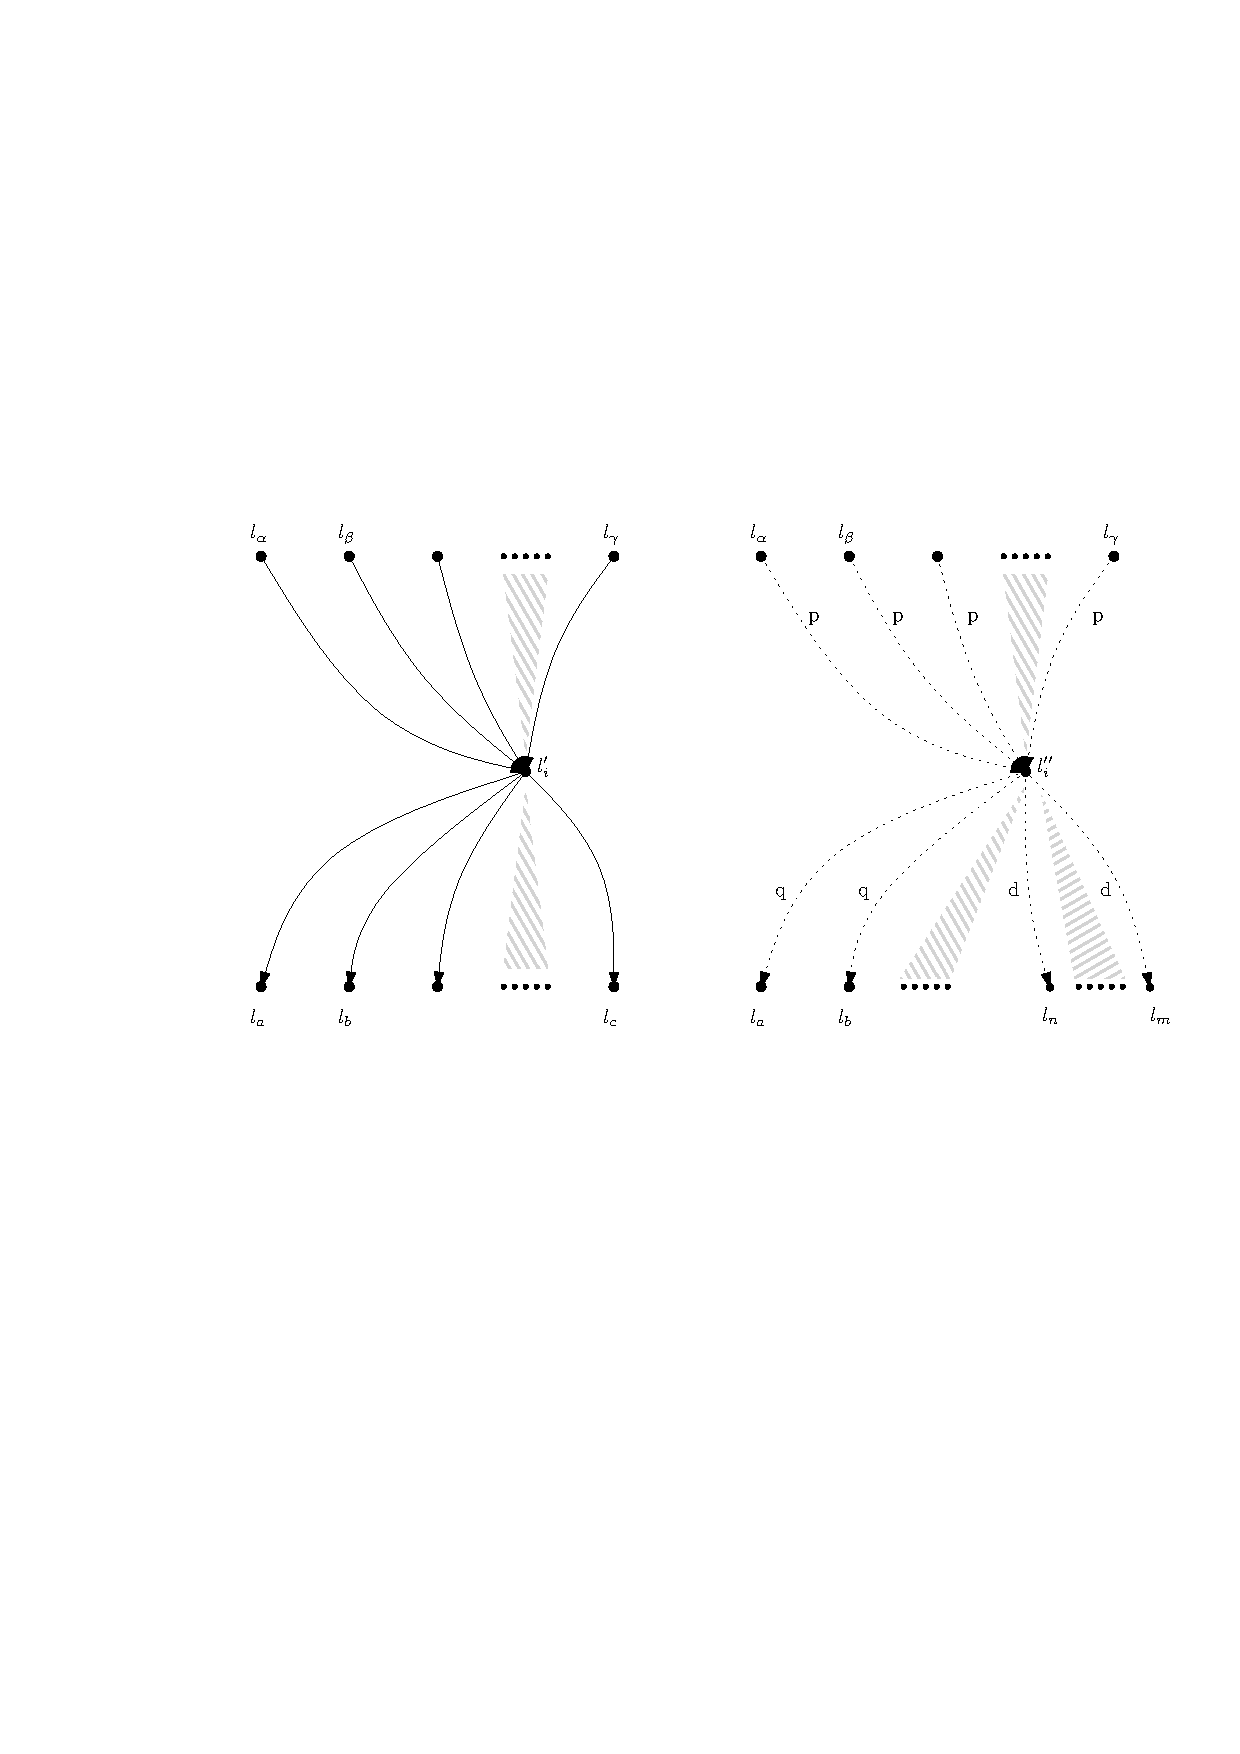
\includegraphics[width=0.8\textwidth]{images/fwspec2p}
		\caption{The rewiring of a species' foodweb neighbourhood during a speciation event in the niche partition model.}
		\label{fig:fwspec2p}
\end{figure}

Another rewiring mechanism for the foodweb during a speciation event is the niche partition model. As before one of the two siblings keep the same place of her ancestor in the foodweb. The active daughter preserves each of her ancestor predator with a probability $p$ (that is, gets rid of it with probability $1-p$) and preserves each prey with probability $q$ (that is, loses it with probability $1-q$). Moreover, the daughter which changing its niche may add new prey in her diet drawing from the set of potential prey $pp_{t}(l_i)$ (which, similarly to what done in the previous model, is the set of species $l_p$ in $C_t$ such that aren't paths from $l_p$ to $l_i$). The active daughter add each species in $pp_{t}(l_i)$ to her diet with probability $$d = \frac{k}{|pp_t(l_i)|}$$  so that the overall probability of adding at least a new prey is \[ \mathbb{P}(\mbox{add at least one species}) = 1 - \left( 1 - d\right)^{|pp_t(l_i)|} \, . \]  The mechanism is depicted in figure~\ref{fig:fwspec2p}.

\section{Extinction under complex ecological constraints}

The most common simple mathematical model of extinction events are given by the \emph{field of bullets} models and its generalization. A problem closely related is finding the, under a set of properly defined constraints, i.e. a cost/budget bound, the conservation policy maximizing the expected phylogenetic diversity.

A natural generalization of this approach may be given taking into account hybridization events and ecological constraint. Natural question regards the expected Phylogenetic Diversity, its variance and its comparison with the classical models.

Insights can be gathered from both a pure analytical approach, working with artificial data, and from the application of the models to empirical observed species community. Preliminary results shows that the behaviour of models where the extinction depends on ecological constraints and hybridization events are allowed is sensibly different from the classical models.

We just show briefly two possible initial model, which will be developed during the thesis research. 

\subsection*{clade size weighted extinction}
Very poor branches of the tree of life, such as just saved from extinction species or small isolated population may have lower probability to survive from a changing habitat.

We propose a model of random extinction which takes into account this issue.

Let $\tau$ be the phylogeny we are considering and $x_i$ its leaves We will call $C^0_r$ and $C^0_l$ the two principal clades at time $0$.

At each extinction event either a species or a clade goes extinct. To select which one to prune we think of extinction as an event running from the root to the leaves and stopping randomly. At each bifurcation the events steps on, it choose to stop with probability
$$\mathbb{P}(\mbox{stops at }C^y)=\left(\frac{1}{|C^y|}\right)^\alpha$$
or decides to proceed on the right or left clade with probability
$$\mathbb{P}(C^y_r)=\left(\frac{|C^y_r|}{|C^y_l|}\right)^\beta \mathbb{P}(C^y_l)$$

where $C^y_r$ ($C^y_l$) is one of the two principal clades descending from $C^y$. A more precise notation can be given registering the $r$ and $l$ path followed in order to come to $C^y$.

When the extinction walk ends, all the species descending from the selected node go extinct.

In general, varying the values of $\beta$ and $\alpha$ (as long as they're both positive), a continuous of scenario where isolated branches goes extinct can be modeled. Notice that if $\alpha \to \infty$ and $\beta = 0$ then the model is simply the classic Field of Bullets model.

\subsection*{Survival through hybridization}

\paragraph{Motivation}

Let's consider a very simple case where we observe two groups of closely related taxa $(A,B)$ and $(B,C)$. Each of them have almost null probability of survival if they are not chosen for a conservation policy and probability $p$ of survival otherwise. Moreover there's a probability $H(A,\neg B)$ that the clade $(A,B)$ generate an hybrid $h_ab$ when $A$ is protected but $B$ is not; there's a probability $H(A,B)$ that the clade $(A,B)$ generate an hybrid $h_{ab}$ when both $A$ and $B$ are protected; there's a probability $H(\neg A, \neg B)$ that the clade $(A,B)$ generate an hybrid $h_{ab}$ when both $A$ and $B$ are not protected. We'll use a similar notation for the clade $(C,D)$ or for hybrid coming from a couple of non-closely related species (as $A$ and $D$ or $B$ and $C$, which are not considered in the Becker et al. paper).

Notice that, without hybridization, protecting the species $A$ and $C$ (scenario 1) brings to a greater expected biodiversity than saving species $A$ and $B$ (scenario 2). On the other hand, if we allow for hybridization events, the previous inequality can be shown to be no more valid.

We will now analyze the expected Phylogenetic Diversity scenario, in the case with hybridization, in the spirit of Becker et al. A careful choice should be made when defining the weight of a hybrid species. We will introduce our choice with a suitable example.

\begin{figure}[h]
	\centering
		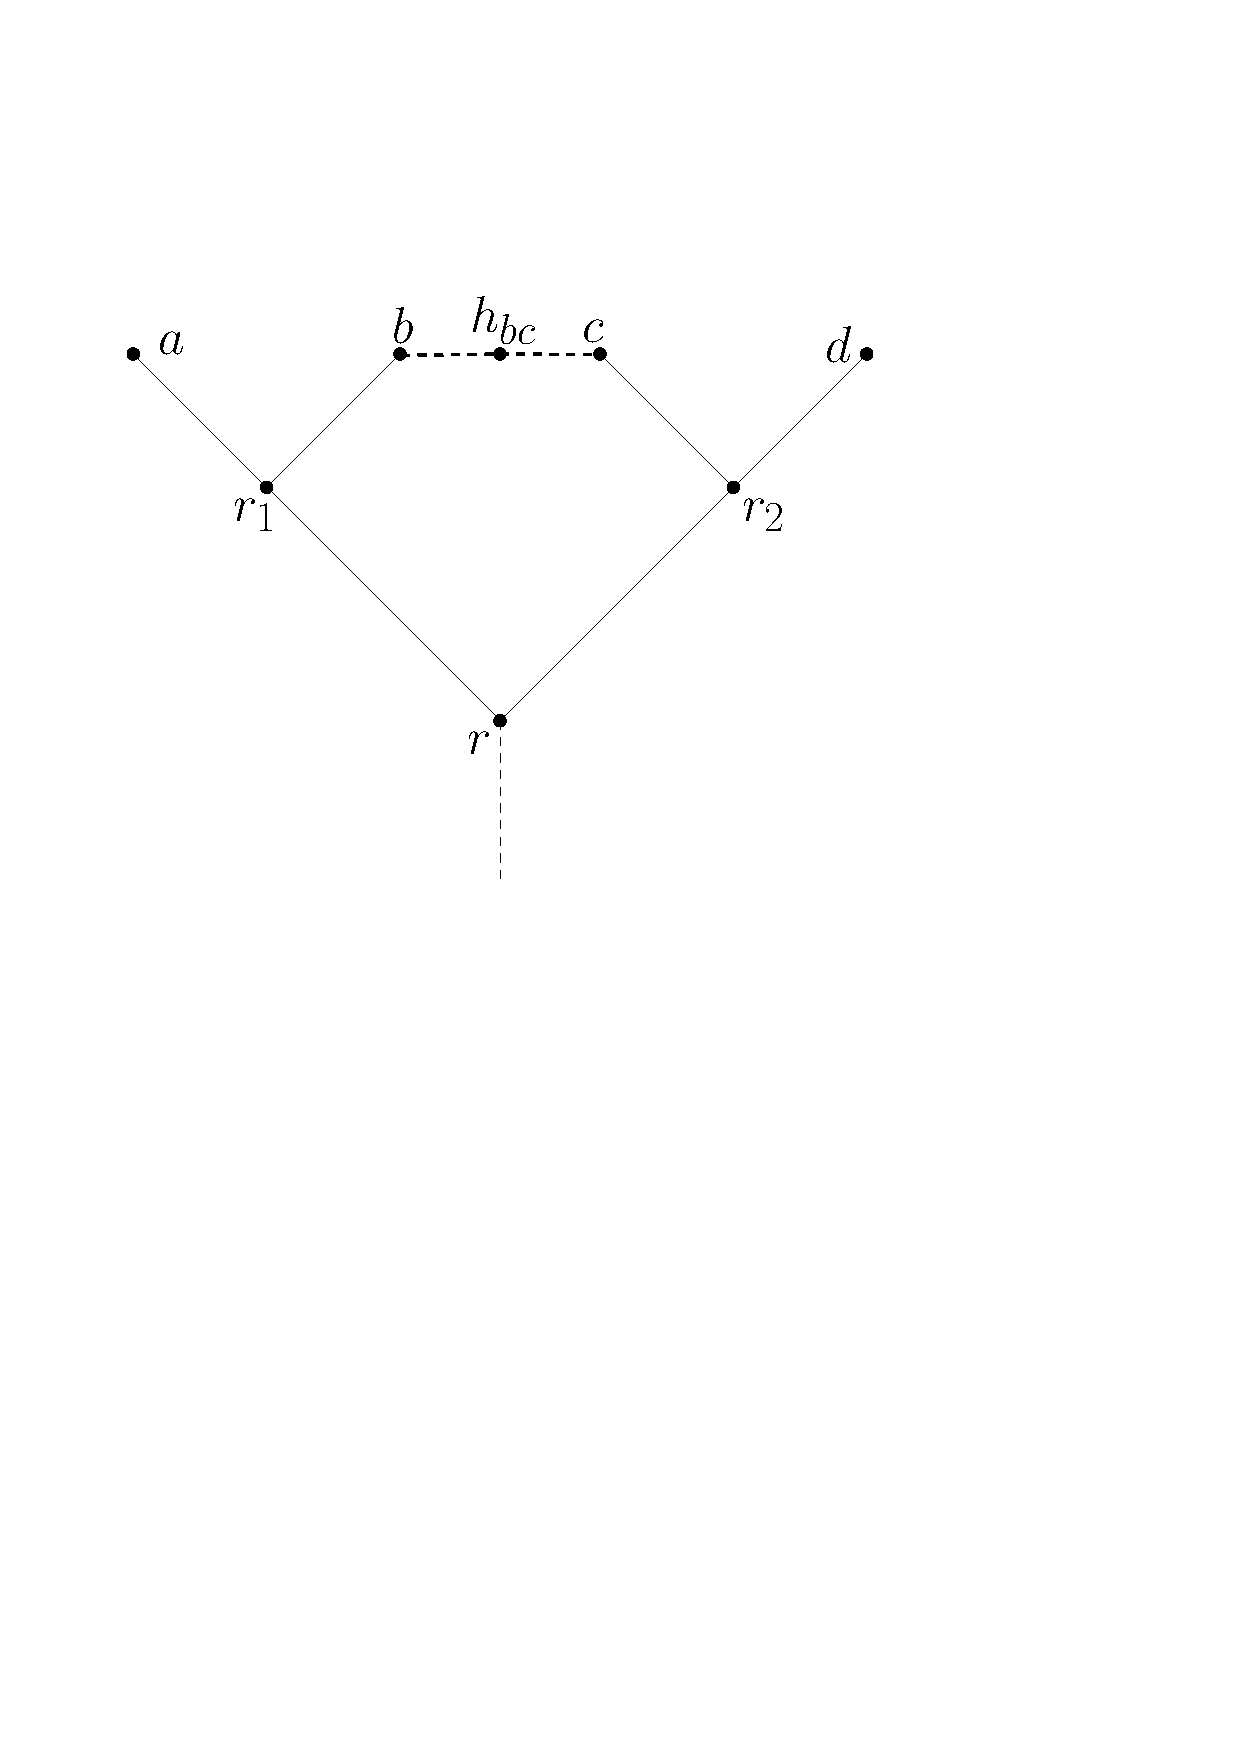
\includegraphics[width=0.5\textwidth]{images/hybridbc}
		\caption{A phylogenetic tree where the species $B$ and $C$ generated an hybrid $h_{bc}$.}
		\label{fig:hybridbc}
\end{figure}

\paragraph{Shared history proportion}
Let $h_{bc}$ be a hybrid generated by the species $B$ and $C$, as in figure~\ref{fig:hybridbc}. The hybrid will inherit a certain proportion of the genetic sequence of $B$, while the remaining part will be inherited from $C$. Let $\delta$ be the proportion of the genetic sequence of $h_{bc}$ coming from $B$, we will write $h_{bc}=\delta C + (1-\delta)B$, with $0 < \delta <1$.

When computing the expected PD, we will consider that a part of the evolutionary history of $C$ is conserved in $h_{bc}$, precisely a proportion equal to $\delta$, and, at the same time a proportion $(1-\delta$ of the evolutionary history of $B$ is conserved in $h_{bc}$. These can be expressed imposing that the branch connecting $h_{bc}$ to $C$ is attached at a $\delta$ of its length, as in figure~\ref{fig:hybridbcdeltalambda}.

\begin{figure}[h]
	\centering
		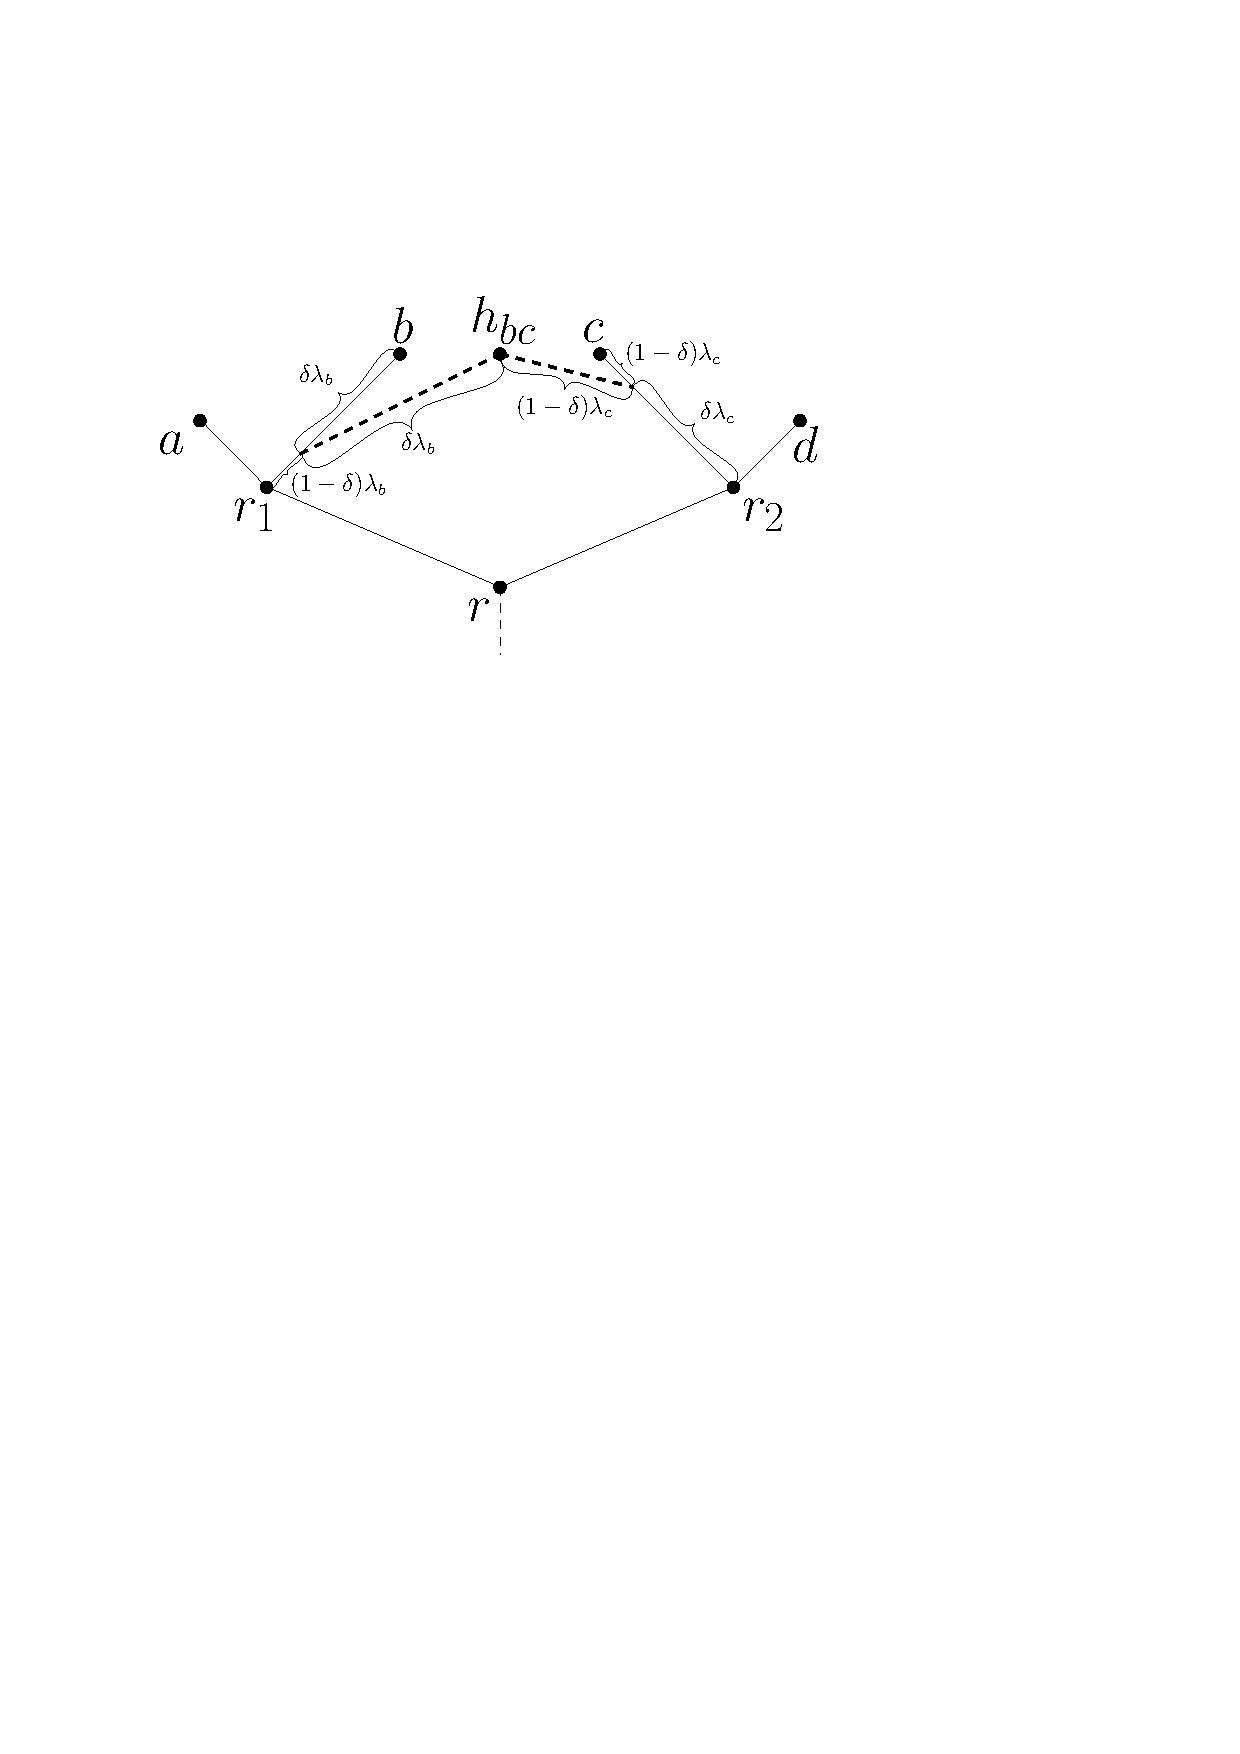
\includegraphics[width=0.7\textwidth]{images/hybridbcdeltalambda}
		\caption{The hybrid $h_{bc}$ conserve $\delta$ ($(1-\delta)$) of the evolutionary history of species $C$ ($B$), nearby the branches we show their length.}
		\label{fig:hybridbcdeltalambda}
\end{figure}

Given the length of the various branches in the original phylogeny (the one without the hybrid) and the survival probability for each of the extant species (and the hybrids), it is straightforward to compute the expected Phylogenetic Diversity of the tree.

We will model hybridization through a random process occurring with a probability depending on the evolutionary history of the species \[\mathbb{P}(H(i,j))=\frac{1}{\mbox{k } d(i,j)}\] where $k$ is a scale factor ($\mbox{k}\geq 1$), $d(i,j)$ is the phylogenetic distance between species $i$ and $j$ normalized so that the shortest branch in the phylogeny has length $1$, so to have $\min_{i,j}(d(i,j)) \geq 2$. Moreover, if a species is extinct or doomed, that is, has zero survival probability, its probability to generate a hybrid is also zero.

In the case where a hybrid may be originated, its PD contribution will be weighted by both the hybridization probability, $H(i,j)$, and the survival probability, $p_h$, of the hybrid. 

\appendix
\chapter{Work Plan}
\begin{figure}[h]
		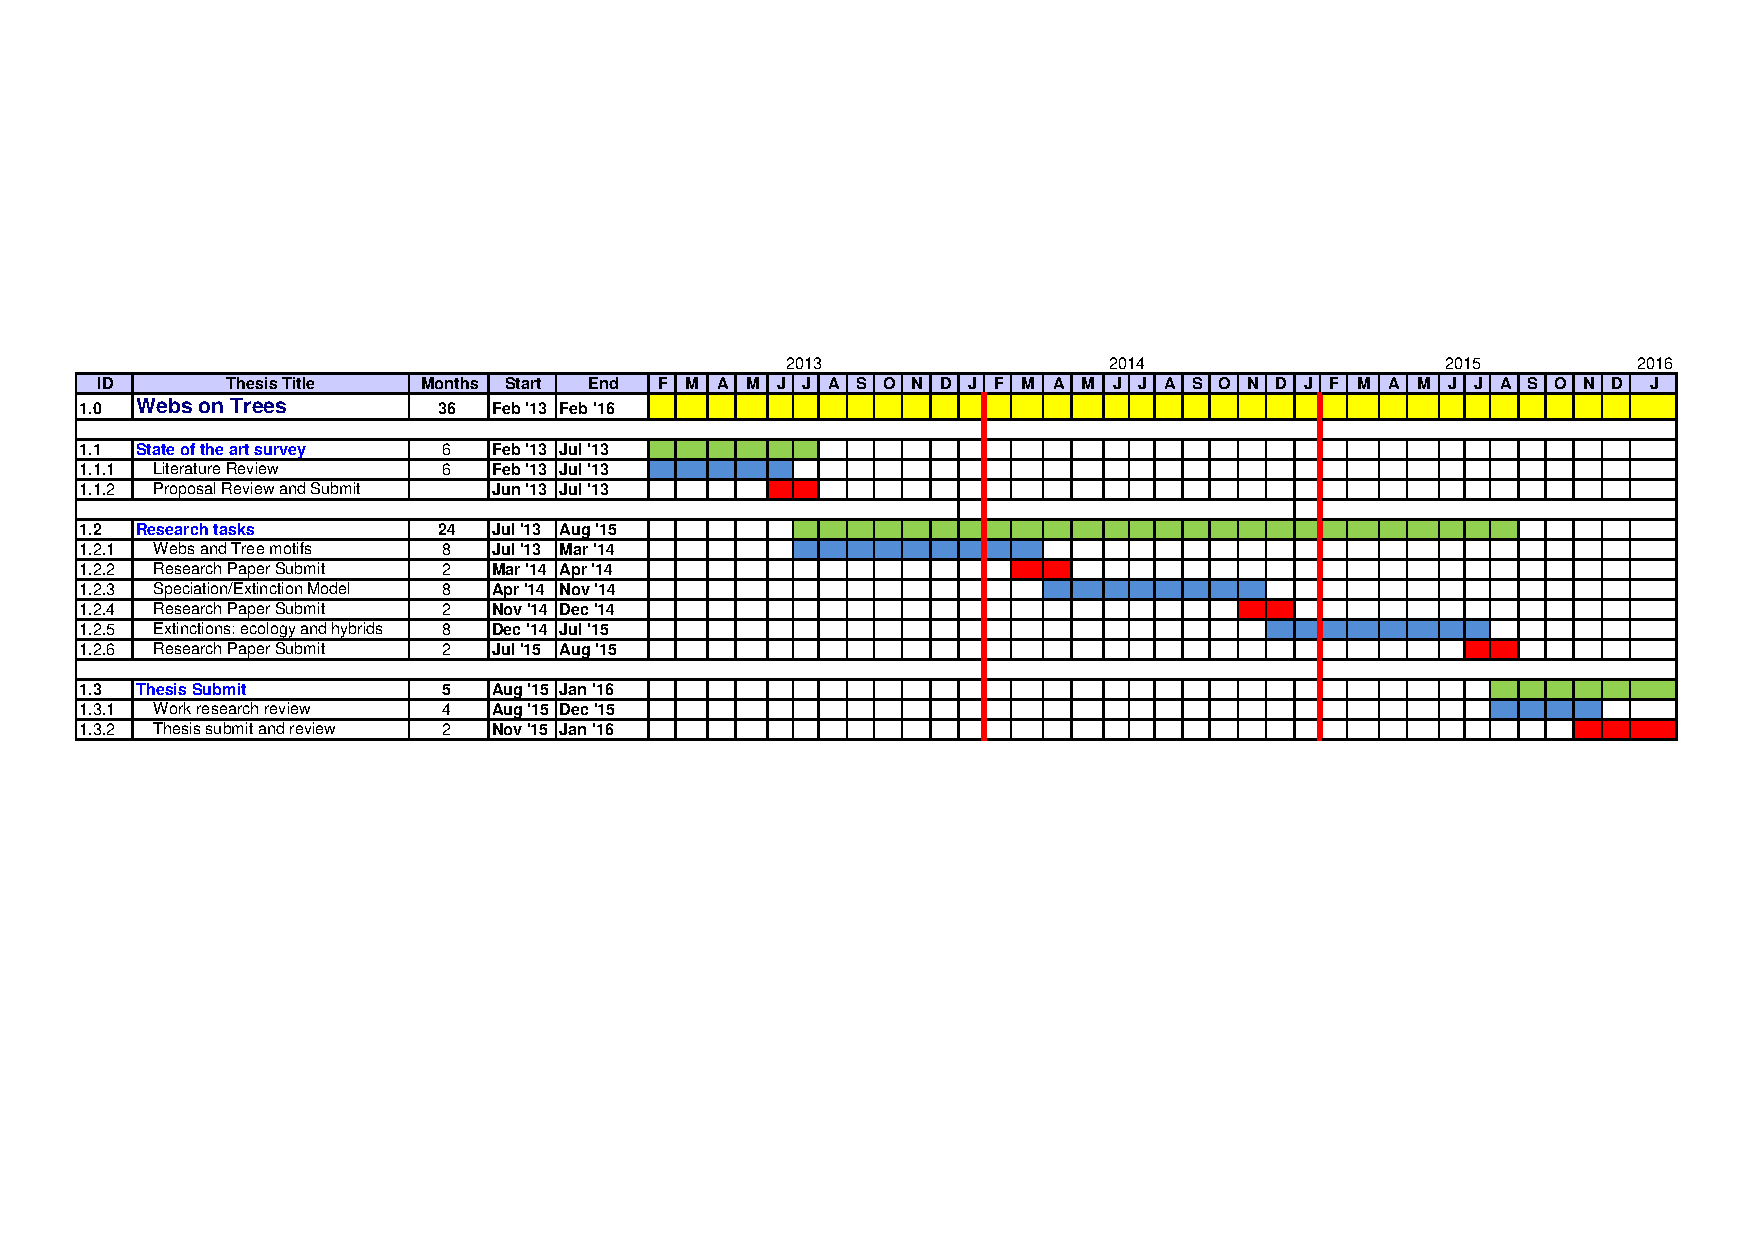
\includegraphics[width=\textwidth]{images/PhD_gantt_center}
		\caption{Gantt diagram of the PhD work tasks. See last page for better resolution}
\end{figure}

\begin{small}
\bibliographystyle{siam}
\bibliography{research_proposal}
\end{small}

\begin{figure}[h]
		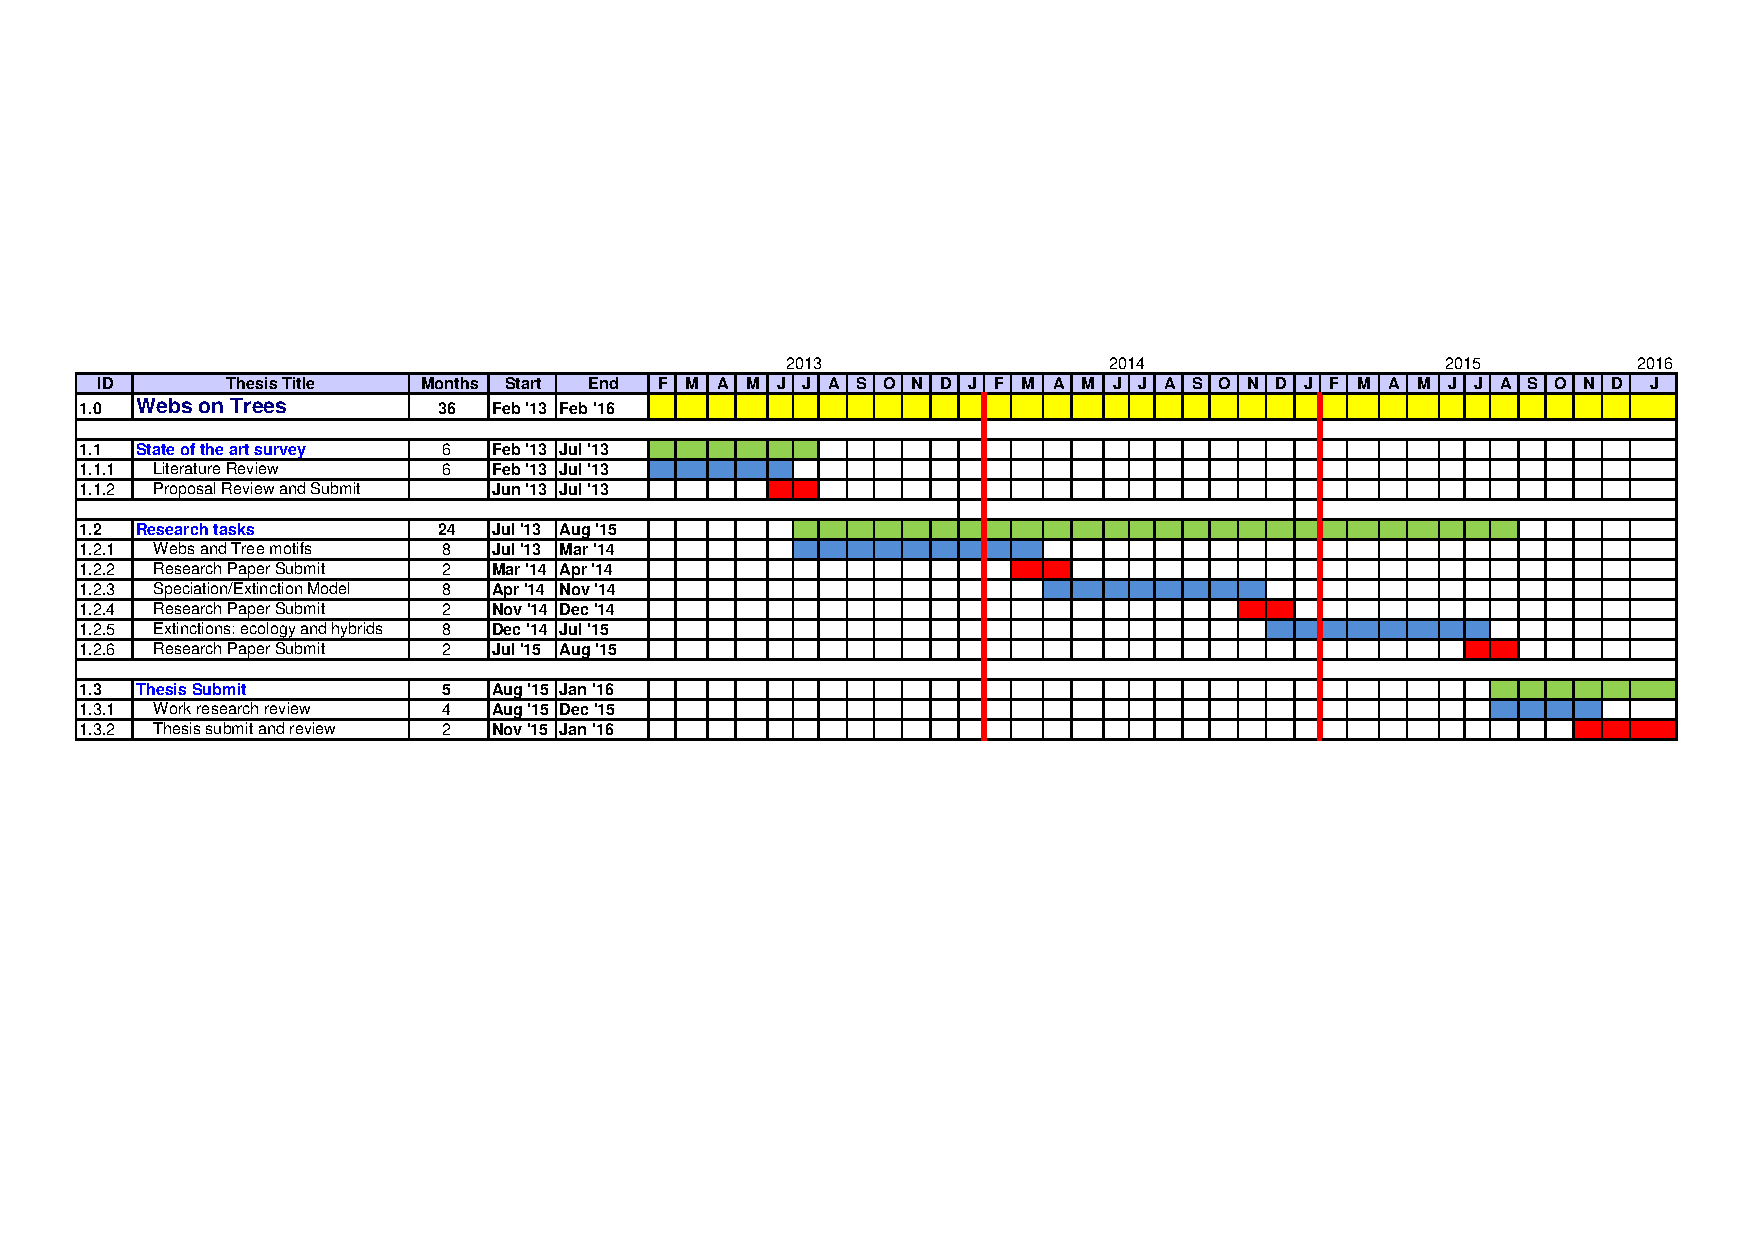
\includegraphics[width=1.6\textwidth, angle=90]{images/PhD_gantt_center}
\end{figure}

\end{document}
